\chapter{The Vision Package} \label{vision-chapter}
The {\bf vision} package includes some higher level image manipulation
routines.
To be able to use any routine or structure in the vision package
use the declaration
\begin{verbatim}
      #include <gandalf/vision.h>
\end{verbatim}
but including individual module header files instead will speed up program
compilation.

\section{Cameras} \label{camera-sec}
The camera modules are separated into single and double precision versions.
The double precision camera structure is defined in
\begin{verbatim}
      #include <gandalf/vision/camera.h>
\end{verbatim}
and the single precision version in
\begin{verbatim}
      #include <gandalf/vision/cameraf.h>
\end{verbatim}
The Gandalf camera defines the transformation from camera 3D coordinates
into image coordinates and back again. Ten camera models are defined,
all using the assumption that the projected position in the image is
independent of the depth.
The camera structure (double precision floating point version) is as follows:
\begin{verbatim}
      /**
        * \brief Structure containing camera parameters.
        */
      typedef struct Gan_Camera
      {
         /// Type of camera
         Gan_CameraType type;

         /// parameters of linear camera

         /// focal distance in x/y pixels
         double fx, fy;

         /// image centre x/y coordinates
         double x0, y0;

         /// third homogeneous image coordinate
         double zh;

         /**
          * \brief Supplementary parameters for non-linear camera models.
          *
          * The thresholds are the square \f$ R^2 \f$ of the undistorted radial
          * camera coordinate \f$ R \f$ where the first reversal of distortion occurs
          * (\a thres_R2), and the similar threshold on the distorted radial
          * distance \f$ d\:R \f$, involving both the distortion coefficient
          * \f$ d \f$  and \f$ F \f$ (thres_dR), at the same reversal point.
          * Both thresholds are set to \c DBL_MAX if there is no reversal.
          */
         union
         {
            struct
            {
               /// Distortion coefficients
               double K1;
      
               /// Thresholds on \f$ R^2 \f$ and \f$ d\:R \f$
               double thres_R2, thres_dR;
      
               /// Outer linear model parameters
               double outer_a, outer_b;
            } radial1;
      
            struct
            {
               /// Distortion coefficients
               double K1, K2;
      
               /// Thresholds on \f$ R^2 \f$ and \f$ d\:R \f$
               double thres_R2, thres_dR;
      
               /// Outer linear model parameters
               double outer_a, outer_b;
            } radial2;
      
            struct
            {
               /// Distortion coefficients
               double K1, K2, K3;
      
               /// Thresholds on \f$ R^2 \f$ and \f$ d\:R \f$
               double thres_R2, thres_dR;
      
               /// Outer linear model parameters
               double outer_a, outer_b;
            } radial3;
      
            struct { double cxx, cxy, cyx, cyy; } xydist4;
         } nonlinear;

         /// gamma value of images taken using this camera
         double gamma;

         /// point functions
         struct
         {
            /// point projection function
            Gan_Bool (*project) ( struct Gan_Camera *camera,
                                  Gan_Vector3 *X, Gan_Vector3 *p,
                                  Gan_Matrix22 *HX, struct Gan_Camera HC[2],
                                  int *error_code );

            /// point back-projection function
            Gan_Bool (*backproject) ( struct Gan_Camera *camera,
                                      Gan_Vector3 *p, Gan_Vector3 *X,
                                      int *error_code );

            /// function to add distortion to a point
            Gan_Bool (*add_distortion) ( struct Gan_Camera *camera,
                                         Gan_Vector3 *pu, Gan_Vector3 *p,
                                         int *error_code );

            /// function to remove distortion from a point
            Gan_Bool (*remove_distortion) ( struct Gan_Camera *camera,
                                            Gan_Vector3 *p, Gan_Vector3 *pu,
                                            int *error_code);
         } point;

         /// line functions
         struct
         {
            /// line projection function
            Gan_Bool (*project) ( struct Gan_Camera *camera,
                                  Gan_Vector3 *L, Gan_Vector3 *l );

            /// line back-projection function
            Gan_Bool (*backproject) ( struct Gan_Camera *camera,
                                      Gan_Vector3 *l, Gan_Vector3 *L );
         } line;
      } Gan_Camera;
\end{verbatim}
The single precision version {\tt Gan\_Camera\_f} is defined similarly.
The camera models are defined in {\tt <gandalf/vision/camera\_defs.h>},
and are
\begin{verbatim}
      /**
       * \brief Camera models supported by Gandalf.
       */
      typedef enum
      {
         /// linear camera model
         GAN_LINEAR_CAMERA,

         /// one parameter K1 of radial distortion
         GAN_RADIAL_DISTORTION_1,

         /// two parameters K1,K2 of radial distortion
         GAN_RADIAL_DISTORTION_2,

         /// three parameters K1,K2,K3 of radial distortion */
         GAN_RADIAL_DISTORTION_3,

         /// one parameter K1 of inverse radial distortion
         GAN_RADIAL_DISTORTION_1_INV,

         /// stereographic projection
         GAN_STEREOGRAPHIC_CAMERA,

         /// equidistant projection
         GAN_EQUIDISTANT_CAMERA,

         /// sine-law projection
         GAN_SINE_LAW_CAMERA,

         /// equi-solid angle projection
         GAN_EQUI_SOLID_ANGLE_CAMERA,

         /// distortion model as used by 3D Equalizer V4
         GAN_XY_DISTORTION_4,
      } Gan_CameraType;
\end{verbatim}
The linear and radial distortion models are standard models.
The stereographic, equidistant, sine law and equi-solid angle models are
wide-angle camera models from~\cite{Fleck:TR94}.

The coordinate frames are illustrated in Figure~\ref{camera}.
\begin{figure}
 \centerline{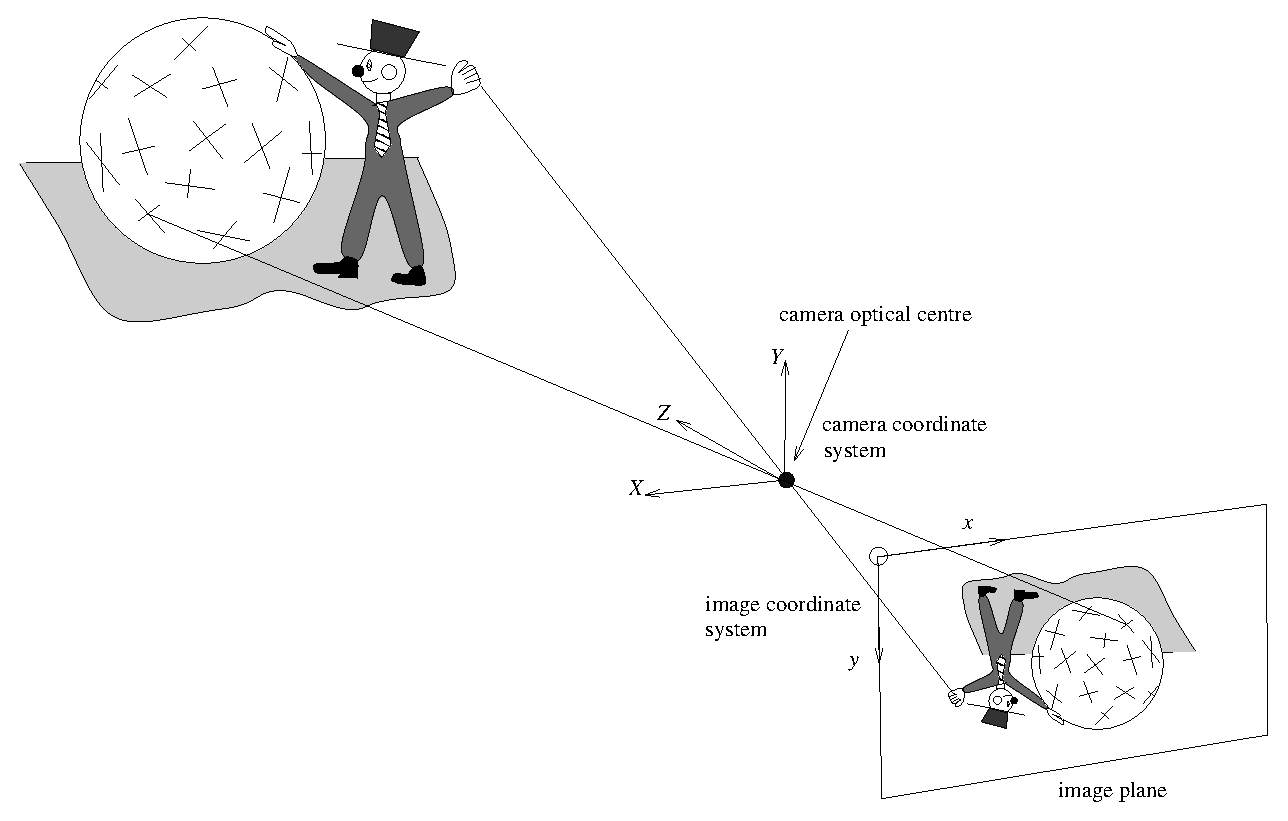
\psfig{file=camera.ps,width=120mm}}
 \caption{Illustration of coordinate frames in projection from camera 3D
          frame into the image.}
 \label{camera}
\end{figure}

The linear camera model is the simplest standard camera model. It defines
the following model relating camera 3D coordinates $X,Y,Z$ to image
coordinates $x,y$:
\begin{equation}
 x = x_0 + f_x\frac{X}{Z},\;\;\;\;y = y_0 + f_y\frac{Y}{Z}
 \label{linear-camera-model}
\end{equation}
This equation derives from the similar triangles apparent in the
geometrical model illustrated in Figure~\ref{project}.
\begin{figure}
 \centerline{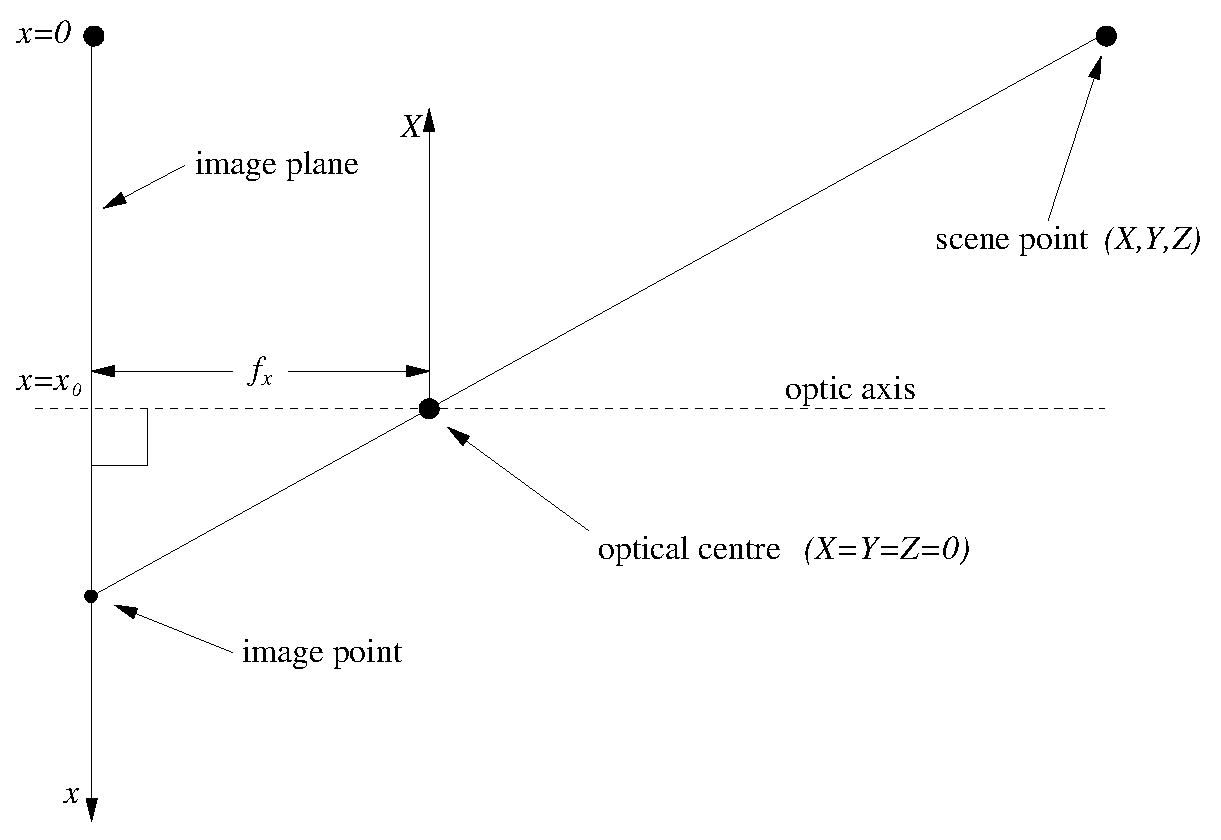
\psfig{file=project.ps,width=120mm}}
 \caption{Geometrical model of projection from camera 3D coordinates $X,Y,Z$
	onto image coordinates $x,y$ for a perfect pinhole camera,
	here showing only the relationship between $X,Z$ and $x$.
	The optic axis is defined as being perpendicular to the image plane
        and intersecting the optical centre of the camera. Note the reversal
	between the 3D camera $X$ axis and the image $x$ axis, caused by
        the projection.}
 \label{project}
\end{figure}
The image centre coordinates $x_0,y_0$ and focal distance parameters $f_x,f_y$
correspond to the similarly named {\tt x0, y0} and {\tt fx, fy} fields in
the {\tt Gan\_Camera} structure. The normal way to write the linear model
is in homogeneous coordinates, introducing the third image coordinate $z_h$,
which can be identified with the {\tt zh} field of the {\tt Gan\_Camera}
structure:
\[ \beginm{l} x \\ y \\ z_h \endm =
   \lambda \beginm{ccc} f_x & 0 & x_0 \\ 0 & f_y & y_0 \\ 0 & 0 & z_h \endm
   \beginm{c} X \\ Y \\ Z \endm\;\;\;\mbox{or}\;\;\;
   \xvec = \lambda K \Xvec
\]
The $\lambda$ parameter can be eliminated, to recover
Equation~\ref{linear-camera-model}.
$z_h$ can be set to one, but a good rule of thumb
is to set it to roughly half the range of image $x/y$ coordinates, so that
all the image coordinates will be scaled in approximately the same way,
which can reduce truncation error in certain situations.
$K$ is known as the {\em camera calibrarion matrix}:
\[ K = \beginm{ccc} f_x & 0 & x_0 \\ 0 & f_y & y_0 \\ 0 & 0 & z_h \endm
\]
Note the units the elements of $K$. $f_x$ and $f_y$ both represent the same
distance, the perpendicular distance from the image plane to the optical
centre, but they are measured in image $x$ and $y$ pixels respectively.
$x_0$ is the position of the image centre in the image $x$ direction and
measured in image $x$ pixels, and similarly for $y_0$. Note also that $f_x$
and $f_y$ do not measure the focal {\em length} of the camera.
The focal length is purely a property of the lens system.
Under normal circumstances the focal distance will be shorter than the
focal length, unless the camera
is focussing at infinity when the two distances will be the same.

The linear model is an ``ideal'' model, corresponding to a perfect pinhole
camera. It is safe to use this model when the focal length of the lens is
large. In practice there will be non-linear distortions, and the
simplest model of distortion is that it is purely {\tt radial},
i.e. directed directly towards or away from the centre of the
image\footnote{In practice the centre of distortion will be somewhat
different from the image centre~\cite{Slama:etal:PHOTOG80}.}
A simple model of this distortion is
\begin{equation}
 x = x_0 + f_x (1+d)\frac{X}{Z},\;\;\;\;y = y_0 + f_y (1+d)\frac{Y}{Z}
 \label{radial-distortion-model}
\end{equation}
where
\[ d = K_1 r^2 + K_2 r^4 + K_3 r^6\;\;\;\;\mbox{and}\;\;\;\;r^2 = \frac{X^2 + Y^2}{Z^2}
\]
Here $d$ represents the non-linear distortion. The camera models
{\tt GAN\_RADIAL\_DISTORTION\_1}, {\tt GAN\_RADIAL\_DISTORTION\_2}
and {\tt GAN\_RADIAL\_DISTORTION\_3}
represent the above distortion model with respectively $K_1$ only,
both $K_1$ \& $K_2$ and all of $K_1$, $K_2$ and $K_3$.
Once a camera has been created, it can be used to project from camera to
image coordinates, or to back-project from image out into camera coordinates.
Note that although the projection is apparently from a 3D space onto a
2D space, you should think instead of a projection between two 2D spaces.
All camera 3D points along a straight line through the optical centre
project to the same image point, so the projection is between the image
plane and the space of {\em rays} in camera 3D space through the optical
centre, a 2D space of rays.

\subsection{Building cameras}
To create a linear camera, you will need the header file
\begin{verbatim}
      #include <gandalf/vision/camera_linear.h>
\end{verbatim}
for double precision or
\begin{verbatim}
      #include <gandalf/vision/cameraf_linear.h>
\end{verbatim}
Then use the routine
\begin{verbatim}
      Gan_Camera CameraD;

      /* build a linear camera in double precision */
      gan_camera_build_linear ( &CameraD,
                             /* ZH     FY     FX     Y0     X0 */
                                100.0, 700.0, 500.0, 150.0, 100.0 );
\end{verbatim}
to create a double precision linear camera.
There is a single-precision camera structure, called
a {\tt Gan\_Camera\_f}. The single precision version of the above function is
\begin{verbatim}
      Gan_Camera_f CameraF;

      /* build a linear camera in double precision */
      gan_cameraf_build_linear ( &CameraF,
                              /* ZH      FY      FX      Y0      X0 */
                                 100.0F, 700.0F, 500.0F, 150.0F, 100.0F );
\end{verbatim}
There are similar functions for creating cameras with a radial distortion
model, for which you will need one or more of the following header files:
\begin{verbatim}
      #include <gandalf/vision/camera_radial_dist1.h>
      #include <gandalf/vision/camera_radial_dist2.h>
      #include <gandalf/vision/camera_radial_dist3.h>
      #include <gandalf/vision/cameraf_radial_dist1.h>
      #include <gandalf/vision/cameraf_radial_dist2.h>
      #include <gandalf/vision/cameraf_radial_dist3.h>
\end{verbatim}

Then the functions are
\begin{verbatim}
      /* build a camera with one radial distortion parameter */
      gan_camera_build_radial_distortion_1 ( &CameraD,
                                       /*    ZH     FY     FX     Y0     X0 */
                                             100.0, 700.0, 500.0, 150.0, 100.0,
                                       /*    K1 */
                                             0.001 ); /* OR */
      gan_cameraf_build_radial_distortion_1 ( &CameraF,
                                        /*    ZH      FY      FX      Y0      X0 */
                                              100.0F, 700.0F, 500.0F, 150.0F, 100.0F,
                                        /*    K1 */
                                              0.001F );

      /* build a camera with two radial distortion parameters */
      gan_camera_build_radial_distortion_2 ( &CameraD,
                                       /*    ZH     FY     FX     Y0     X0 */
                                             100.0, 700.0, 500.0, 150.0, 100.0,
                                       /*    K1,    K2 */
                                             0.001, 1.0e-7 ); /* OR */
      gan_cameraf_build_radial_distortion_2 ( &CameraF,
                                        /*    ZH      FY      FX      Y0      X0 */
                                              100.0F, 700.0F, 500.0F, 150.0F, 100.0F,
                                        /*    K1,     K2 */
                                              0.001F, 1.0e-7F );
      /* build a camera with three radial distortion parameters */
      gan_camera_build_radial_distortion_3 ( &CameraD,
                                       /*    ZH     FY     FX     Y0     X0 */
                                             100.0, 700.0, 500.0, 150.0, 100.0,
                                       /*    K1,    K2,     K3 */
                                             0.001, 1.0e-7, -0.0001 ); /* OR */
      gan_cameraf_build_radial_distortion_3 ( &CameraF,
                                        /*    ZH      FY      FX      Y0      X0 */
                                              100.0F, 700.0F, 500.0F, 150.0F, 100.0F,
                                        /*    K1,     K2,      K3 */
                                              0.001F, 1.0e-7F, -0.0001F );
\end{verbatim}
Note that {\tt Gan\_Camera}'s and {\tt Gan\_Camera\_f}'s are simple structures
with no internally allocated data, so there is no {\tt ...\_free} function
for them.

\subsection{Projecting points and lines}
Routines for projecting points and lines into an image are provided.
The double precision routines are
\begin{verbatim}
      Gan_Vector3 v3X, v3x; /* declare camera/scene points X, x */
      Gan_Vector3 v3L, v3l; /* declare camera/scene lines L, l */

      /* fill camera point X & line L with values */
      gan_vec3_fill_q ( &v3X, 1.5, -0.8, 1.2 );
      gan_vec3_fill_q ( &v3L, 2.7,  3.9, 3.6 );

      /* project point from camera 3D coordinates onto the image X --> x */
      gan_camera_project_point_q ( &CameraD, &v3X, &v3x );

      /* project line from camera 3D coordinates onto the image L --> l */
      gan_camera_project_line_q ( &CameraD, &v3L, &v3l );
\end{verbatim}
The point projection function implements the projection
equations~\ref{linear-camera-model} and~\ref{radial-distortion-model}.
The lines are represented in homogeneous 2D coordinates, so that
the line $\Lvec$ in camera coordinates actually describes a {\em plane}
in 3D space intersecting the origin (optical centre). If $\Xvec$ is a
point in camera $X,Y,Z$ space, the line in the homogeneous 2D space of
camera ``rays'' is defined by the equation
\[ \Lvec.\Xvec = 0\;\;\;\;\mbox{or}\;\;\;\; L_X X + L_Y Y + L_Z Z = 0
\]
The line in image coordinates $\xvec=(x\;y\;z_h)\tr$ is similarly defined as
\[ \lvec.\xvec = 0\;\;\;\;\mbox{or}\;\;\;\; l_x x + l_y y + l_z z_h = 0
\]
Projection of lines is only available for linear cameras, since when there
is distortion lines in 3D space project to curves on the image.
For a linear camera the relationship between $\Lvec$ and $\lvec$ is
\[ \lvec = K\trinv\Lvec
\]

There are also versions of the above routines which perform the projection
in-place in the input vector. So for instance
\begin{verbatim}
      Gan_Vector3 v3Xx; /* declare point */
      Gan_Vector3 v3Ll; /* declare line */

      /* fill camera point X & line L with values */
      gan_vec3_fill_q ( &v3Xx, 1.5, -0.8, 1.2 );
      gan_vec3_fill_q ( &v3Ll, 2.7,  3.9, 3.6 );

      /* project point from camera 3D coordinates onto the image in-place */
      gan_camera_project_point_i ( &CameraD, &v3Xx );

      /* project line from camera 3D coordinates onto the image in-place */
      gan_camera_project_line_i ( &CameraD, &v3Ll );
\end{verbatim}

Back-projection from image to camera coordinates operates similarly.
To back-project a point and a line you can use
\begin{verbatim}
      Gan_Vector3 v3X, v3x; /* declare camera/scene points X, x */
      Gan_Vector3 v3L, v3l; /* declare camera/scene lines L, l */

      /* fill image point x & line l with values */
      gan_vec3_fill_q ( &v3x, 1.5, -0.8, 1.2 );
      gan_vec3_fill_q ( &v3l, 2.7,  3.9, 3.6 );

      /* back-project point from the image into camera 3D coordinates x --> X */
      gan_camera_backproject_point_q ( &CameraD, &v3x, &v3X ); /* OR */
      gan_camera_backproject_point_i ( &CameraD, &v3x ); /* in-place */

      /* backproject line from the image into camera 3D coordinates l --> L */
      gan_camera_backproject_line_q ( &CameraD, &v3l, &v3L ); /* OR */
      gan_camera_backproject_line_i ( &CameraD, &v3l ); /* in-place */
\end{verbatim}

The single precision versions of these functions operate similarly.
The single precision camera to image projection functions are
\begin{verbatim}
      Gan_Vector3_f v3X, v3x; /* declare camera/scene points X, x */
      Gan_Vector3_f v3L, v3l; /* declare camera/scene lines L, l */

      /* fill camera point X & line L with values */
      gan_vec3f_fill_q ( &v3X, 1.5F, -0.8F, 1.2F );
      gan_vec3f_fill_q ( &v3L, 2.7F,  3.9F, 3.6F );

      /* project point from camera 3D coordinates onto the image X --> x */
      gan_cameraf_project_point_q ( &CameraF, &v3X, &v3x ); /* OR */
      gan_cameraf_project_point_i ( &CameraF, &v3X ); /* in-place */

      /* project line from camera 3D coordinates onto the image L --> l */
      gan_cameraf_project_line_q ( &CameraF, &v3L, &v3l ); /* OR */
      gan_cameraf_project_line_i ( &CameraF, &v3L ); /* in-place */
\end{verbatim}
The single precision image to camera back-projection functions are
\begin{verbatim}
      Gan_Vector3_f v3X, v3x; /* declare camera/scene points X, x */
      Gan_Vector3_f v3L, v3l; /* declare camera/scene lines L, l */

      /* fill image point x & line l with values */
      gan_vec3f_fill_q ( &v3x, 1.5F, -0.8F, 1.2F );
      gan_vec3f_fill_q ( &v3l, 2.7F,  3.9F, 3.6F );

      /* project point from camera 3D coordinates onto the image X --> x */
      gan_cameraf_backproject_point_q ( &CameraF, &v3x, &v3X ); /* OR */
      gan_cameraf_backproject_point_i ( &CameraF, &v3x ); /* in-place */

      /* project line from camera 3D coordinates onto the image L --> l */
      gan_cameraf_backproject_line_q ( &CameraF, &v3l, &v3L ); /* OR */
      gan_cameraf_backproject_line_i ( &CameraF, &v3l ); /* in-place */
\end{verbatim}

\subsection{Adding/removing camera distortion}
Gandalf also supplies some functions for adding and removing the
image plane distortion from an image point. So for instance
\begin{verbatim}
      Gan_Camera CameraD;
      Gan_Vector3 v3x, v3xu;

      /* build camera with one parameter of radial distortion */
      gan_camera_build_radial_distortion_1 ( &CameraD,
                                       /*    ZH     FY     FX     Y0     X0 */
                                             100.0, 700.0, 500.0, 150.0, 100.0,
                                       /*    K1 */
                                             0.001 );

      /* build image point x assumed to have distortion */
      gan_vec3_fill_q ( &v3x, 50.0, -80.0, 100.0 );

      /* remove distortion from image point x --> xu */
      gan_camera_remove_distortion_q ( &CameraD, &v3x, &v3xu );
\end{verbatim}
removes the distortion from the image point {\tt x}, producing an
undistorted point {\tt xu}. Given the camera 3D point $\Xvec$ that projects
onto {\tt x}, {\tt xu} is defined as the point on the image onto which the
equivalent linear camera (i.e. the linear camera with the same $f_x$, $f_y$,
$x_0$, $y_0$ and $z_h$) would project when applied to $\Xvec$.
The in-place version of this function is
\begin{verbatim}
      /* remove distortion from image point x --> xu in-place */
      gan_camera_remove_distortion_i ( &CameraD, &v3x );
\end{verbatim}

The reverse is to add distortion to an image point. Given a non-linear camera,
this means converting a point projected with the equivalent linear camera
to a point projected with the non-linear camera:
\begin{verbatim}
      /* build image point xu assumed to have NO distortion */
      gan_vec3_fill_q ( &v3xu, 50.0, -80.0, 100.0 );

      /* add distortion to image point xu --> x */
      gan_camera_add_distortion_q ( &CameraD, &v3xu, &v3x ); /* OR */
      gan_camera_add_distortion_i ( &CameraD, &v3xu ); /* in-place */
\end{verbatim}

The single precision versions of these routines are
\begin{verbatim}
      Gan_Camera_f CameraF;
      Gan_Vector3_f v3x, v3xu;

      /* build camera with one parameter of radial distortion */
      gan_cameraf_build_radial_distortion_1 ( &CameraF,
                                        /*    ZH      FY      FX      Y0      X0 */
                                              100.0F, 700.0F, 500.0F, 150.0F, 100.0F,
                                        /*    K1 */
                                              0.001F );

      /* build image point x assumed to have distortion */
      gan_vec3f_fill_q ( &v3x, 50.0F, -80.0F, 100.0F );

      /* remove distortion from image point x --> xu */
      gan_cameraf_remove_distortion_q ( &CameraF, &v3x, &v3xu ); /* OR */
      gan_cameraf_remove_distortion_i ( &CameraF, &v3x ); /* in-place */

      /* build image point xu assumed to have NO distortion */
      gan_vec3f_fill_q ( &v3xu, 50.0F, -80.0F, 100.0F );

      /* add distortion to image point xu --> x */
      gan_cameraf_add_distortion_q ( &CameraF, &v3xu, &v3x ); /* OR */
      gan_cameraf_add_distortion_i ( &CameraF, &v3xu ); /* in-place */
\end{verbatim}

\subsection{Building the camera calibration matrix}
The camera calibration matrix $K$ is triangular. Gandalf provides a
routine to build $K$ from the calibration structure. The double precision
version is
\begin{verbatim}
      Gan_Camera CameraD; /* declare camera structure */
      Gan_SquMatrix33 sm33K; /* declare camera calibration matrix K */

      /* ... build camera using e.g. gan_camera_build_linear() ... */

      /* build camera calibration matrix K */
      sm33K = gan_camera_fill_matrix_s ( &CameraD );
\end{verbatim}
and the single precision version is
\begin{verbatim}
      Gan_Camera_f CameraF; /* declare camera structure */
      Gan_SquMatrix33_f sm33K; /* declare camera calibration matrix K */

      /* ... build camera using e.g. gan_cameraf_build_linear() ... */

      /* build camera calibration matrix K */
      sm33K = gan_cameraf_fill_matrix_s ( &CameraF );
\end{verbatim}
Note that although $K$ is an upper triangular matrix, the routines above
produce a {\em lower} triangular matrix, since that is the only form of
fixed size triangular matrix supported by Gandalf. As explained in
Section~\ref{fixed-size-mat-sec}, Any operations involving upper triangular
matrices can be implemented using implicit transpose of a lower triangular
matrix.

\subsection{Converting cameras between precisions}
It is sometimes necessary to convert from a double precision {\tt Gan\_Camera}
to a single precision {\tt Gan\_Camera\_f} or vice versa. Gandalf provides
two versions of these routines:
\begin{verbatim}
      Gan_Camera   CameraD; /* double precision camera */
      Gan_Camera_f CameraF; /* single precision camera */

      /* ... build CameraD using e.g. gan_cameraf_build_linear() ... */

      /* convert camera from double precision to single precision */
      gan_cameraf_from_camera_q ( &CameraD, &CameraF ); /* OR */
      CameraF = gan_cameraf_from_camera_s ( &CameraD );

      /* convert camera back from single precision to double precision */
      gan_camera_from_cameraf_q ( &CameraF, &CameraD ); /* OR */
      CameraD = gan_camera_from_cameraf_s ( &CameraF );
\end{verbatim}

\section{Computing the fundamental/essential matrix} \label{fun-ess-sec}
\begin{verbatim}
      #include <gandalf/vision/fundamental.h>
      #include <gandalf/vision/essential.h>
\end{verbatim}
The fundamental matrix~\cite{Luong:Faugeras:IJCV96} encodes all the
geometrical constraints available given two images of a rigid scene.
Given two images with point locations $\xvec_1=(x_1\;y_1\;z_h)\tr$ and
$\xvec_2=(x_2\;y_2\;z_h)\tr$ in homogeneous coordinates,
the relationship between image points projected from the same scene point is
\[ \xvec_2\tr F \xvec_1 = 0
\]
$F$ is the $3\times 3$ fundamental matrix. To compute $F$ you can use
multiple point matches to solve the above homogeneous linear equations.
The standard technique is to use pre-conditioning followed by
symmetric matrix eigendecomposition to solve for the nine elements of
$F$ up to an undetermined scale factor. 

\begin{verbatim}
      Gan_SymMatEigenStruct SymEigen;
      Gan_Vector3 *av3Point1, *av3Point2; /* arrays of image points */
      Gan_Matrix33 m33F;

      /* allocate arrays of image coordinates, one array for each image */
      av3Point1 = gan_malloc_array ( Gan_Vector3, 100 );
      av3Point2 = gan_malloc_array ( Gan_Vector3, 100 );

      /* ... fill arrays av3Point1 and av3Point2 with point correspondence
             data for 100 points ... */

      /* create structure for computing eigenvalues and eigenvectors,
         initialising accumulated matrix S (here 9x9) to zero */
      gan_symeigen_form ( &SymEigen, 9 );

      /* solve for fundamental matrix */
      gan_fundamental_matrix_fit ( av3Point1, av3Point2, 100, &SymEigen, &m33F );

      /* free stuff */
      gan_symeigen_free ( &SymEigen );
      gan_free_va ( av3Point2, av3Point1, NULL );
\end{verbatim}

The essential matrix $E$ is the equivalent of the fundamental matrix in the
case of known camera calibration parameters. In this case the rotation between
the cameras can be computed, and also the translation vector between them
up to an unknown scale factor. The mathematical model is that the images
are related by the equation
\[ {\xvec_2'}\tr E \xvec_1' = 0
\]
involving the essential matrix $E$, where $\xvec_1'$, $\xvec_2'$ are
{\em ideal} image coordinates for images 1 \& 2, transformed from the
original image coordinates $\xvec_1$, $\xvec_2$ so that $\xvec_1'$ and
$\xvec_2'$ are the projected coordinates for an {\em ideal camera}, which
is to say a linear camera with focal distances $f_x=f_y=1$, image
centre $x_0=y_0=0$, and homogeneous $z$-coordinate $z_h=1$.
The camera calibration matrix for an ideal camera is $K=I_{3\times 3}$.
This means that the 3D camera coordinate frame can be identified with
the ideal image frame (up to scale as usual).
The essential matrix can be written as
\[ E = R[\Tvec]_\times
\]
where $R$ is the rotation matrix, $\Tvec$ is the translation vector
between the camera positions and $[\Tvec]_\times$ is the ``cross product
matrix'' of $\Tvec$, defined as
\[ \Tvec = \beginm{c} T_X \\ T_Y \\ T_Z \endm,\;\;\;\;
   [\Tvec]_\times = \beginm{ccc} 0 & -T_Z & T_Y \\ T_Z & 0 & -T_X \\
   -T_Y & T_X & 0 \endm.
\]
It is termed the cross product matrix because given any 3-vectors $\xvec$
and $\yvec$, $[\xvec]_\times \yvec = \xvec \times \yvec$.
For more details of the essential matrix see~\cite{Faugeras:93}.

The main difference in Gandalf between computing the fundamental and essential
matrices is in the computation of the ideal image coordinates.
These can be computed by back-projecting the original image coordinates
out into 3D camera (ideal image) coordinates, using the Gandalf
back-projection function described in Section~\ref{camera-sec}.
Here is a code fragment to compute the essential matrix, represented
by the rotation $R$ and translation $\Tvec$.
\begin{verbatim}
      Gan_SymMatEigenStruct SymEigen;
      Gan_Vector3 *av3Point1, *av3Point2; /* arrays of image points */
      Gan_Camera Camera;
      Gan_Euclid3D Pose;

      /* allocate arrays of image coordinates, one array for each image */
      av3Point1 = gan_malloc_array ( Gan_Vector3, 100 );
      av3Point2 = gan_malloc_array ( Gan_Vector3, 100 );

      /* ... fill arrays av3Point1 and av3Point2 with point correspondence
             data for 100 points ... */

      /* build a camera with two radial distortion parameters */
      gan_camera_build_radial_distortion_2 ( &Camera,
                                             100.0, 700.0, 500.0, 150.0, 100.0,
                                             0.001, 1.0e-7 );
      
      /* create structure for computing eigenvalues and eigenvectors,
         initialising accumulated matrix S (here 9x9) to zero */
      gan_symeigen_form ( &SymEigen, 9 );

      /* compute essential matrix */
      gan_essential_matrix_fit ( av3Point1, av3Point2, 100, &Camera, &Camera,
                                 &SymEigen, &Pose );

      /* free stuff */
      gan_symeigen_free ( &SymEigen );
      gan_free_va ( av3Point2, av3Point1, NULL );
\end{verbatim}
The Gandalf 3D Euclidean transformation structure {\tt Gan\_Euclid3D} is
used to store the result rotation and translation.

{\bf Error detection:} Both fundamental and essential matrix routines return
a boolean value, which is {\tt GAN\_FALSE} on error, invoking the Gandalf
error handler.

\section{Computing a homography between 2D scene and image}
\begin{verbatim}
      #include <gandalf/vision/homog33_fit.h>
\end{verbatim}
If a part of the viewed scene is planar, or the camera is undergoing a
pure rotation (or both), the (part of the) scene can be reconstructed
using 2D methods. Here we assume a point-cloud representation, so
the scene is represented by $n$ points $\Xvec_i$ in homogeneous
coordinates, $i=1,\ldots,n$. The relationship between the $\Xvec_i$
and points $\xvec_i$ in an image of the same (part of the) scene is a simple
linear projective transformation or homography:
\begin{equation}
 \xvec_i = \lambda_i P \Xvec_i
 \label{point-proj-eq}
\end{equation}
$P$ is a $3\times 3$ matrix representing the homography and
$\lambda$ is a scale factor. This equation also assumes that the camera
employed in projecting the points onto the image is linear, but if the
camera is non-linear AND the camera parameters are known, the distortion
can be removed first by applying the function
{\tt gan\_camera\_remove\_distortion\_[qi]()} to the image points $\xvec_i$
as described in Section~\ref{camera-sec}.
Given four or more point correspondences
in the image (in general position), the homography matrix $P$ can be computed.
This can be done by first eliminating $\lambda$ to obtain homogeneous
linear equations for the elements of $P$.
Given that $\Xvec=(X\;Y\;Z)\tr$ and $\xvec=(x\;y\;z_h)\tr$,
we can obtain the equations
\begin{equation}
 x \Pvec_3.\Xvec - z_h \Pvec_1.\Xvec = 0,\;\;\;
 y \Pvec_3.\Xvec - z_h \Pvec_2.\Xvec = 0
 \label{homog-point}
\end{equation}
where $P$ is separated into rows as
\[ P = \beginm{c} \Pvec_1\tr \\ \Pvec_2\tr \\ \Pvec_3\tr \endm
\]
From four points we get eight such equations, which allows $P$ to be
computed up to a scale factor using the same symmetric eigensystem routines
as are used to solve for the fundamental and essential matrices above.

Note that this formulation differs from the normal formulation which
considers the homographies {\em between} images. That is a special case
of our formulation, because we can take an image as the projective
``scene'' representation $\Xvec_i$. The scene/image formulation also
allows us to represent the motion over a sequence of $k$ images in 
a compact way as the set of homographies $P\brj$ for images $j=1,\ldots,k$
mapping the scene $\Xvec_i$ to each set of image points $\xvec_i\brj$,
rather than as an arbitrary collection of pairwise homographies.

To start the calculation, define an accumulated symmetric matrix eigensystem
structure and initialise it using the following routine:
\begin{verbatim}
      Gan_SymMatEigenStruct SymEigen;

      /* initialise eigensystem matrix */
      gan_homog33_init ( &SymEigen );  
\end{verbatim}
Then for each point correspondence, build the equations~\ref{homog-point}
and increment the accumulated symmetric eigensystem matrix
by calling the following function:
\begin{verbatim}
      int iEqCount=0, iCount;
      Gan_Vector3 v3X, v3x; /* declare scene and image points X & x */

      for ( iCount = 0; iCount < 100; iCount++ )
      {
         /* ... build scene and image point coordinates into X and x ... */

         /* increment matrix using point correspondence */
         gan_homog33_increment_p ( &SymEigen, &v3X, &v3x, 1.0, &iEqCount );
      }
\end{verbatim}
The fourth argument {\tt 1.0} is a weighting factor for the equations as
described in Section~\ref{acc-symeigen-sec}. The last argument {\tt iEqCount}
is a running count of the total number of equations processed thus far,
to be passed below to the function to solve for $P$.

Once the point correspondences have been processed in this way,
you can solve the equations using
\begin{verbatim}
      Gan_Matrix33 m33P; /* homography matrix P */

      gan_homog33_solve ( &SymEigen, iEqCount, &m33P );
\end{verbatim}
to compute the homography $P$. If you want to repeat the calculation of
a homography with new data, you can start again by calling
\begin{verbatim}
      gan_homog33_reset ( &SymEigen );
\end{verbatim}

At the end of the homography calculation(s) you can free the eigensystem
structure using the function
\begin{verbatim}
      gan_homog33_free ( &SymEigen );
\end{verbatim}

Given correspondences between lines, it is also possible to generate
homogeneous linear equations for $P$ and either combine with points or
compute $P$ purely from lines. To see how to derive the equations for
lines, take the line equations
\[ \Lvec.\Xvec = 0,\;\;\;\;\lvec.\xvec = 0
\]
define the homogeneous line parameters $\Lvec$ in the scene and $\lvec$ in
the image. We can derive the relationship between $\Lvec$, $\lvec$ and $P$
using the point projection equation~\ref{point-proj-eq}, yielding
\[ \Lvec = \mu P\tr \lvec
\]
for a scale factor $\mu$. Separating $P$ into columns as
\[ P = \beginm{ccc} \Pvec'_1 & \Pvec'_2 & \Pvec'_3 \endm,
\]
eliminating $\mu$ from the above equation, and writing
$\Lvec = (L_X\;L_Y\;L_Z)\tr$, we obtain the two homogeneous linear equations
\[ L_X \Pvec'_3.\lvec = L_Z \Pvec'_1.\lvec,\;\;\;
   L_Y \Pvec'_3.\lvec = L_Z \Pvec'_2.\lvec.
\]
Given correspondence between a known scene line $\Lvec$ and a known image
line $\lvec$, the following routine generates these equations and
accumulates them in the calculation of $P$:
\begin{verbatim}
         Gan_Vector3 v3L, v3l; /* declare scene line L and image line l */

         /* ... fill L and l with values for corresponding lines ... */

         /* increment matrix using line correspondence */
         gan_homog33_increment_l ( &SymEigen, &v3L, &v3l, 1.0, &iEqCount );
\end{verbatim}

This is assuming that the endpoints of the scene line are unknown. In practice
the scene line will normally be created from previous matching of image
lines, which are line {\em segments}, so that the endpoints $\Xvec_1$ and
$\Xvec_2$ of the line in scene coordinates will be approximately known.
Note that we don't depend on locating the actual endpoints of the line
accurately, which is a notoriously difficult problem. You should think of
the two points $\Xvec_1$ and $\Xvec_2$ instead as {\em representative}
points on the line. In this case
there is an alternative way of incorporating the line information which
seems to give better numerical performance. We note that the scene line
endpoints $\Xvec_1$ and $\Xvec_2$ should project onto the image line $\lvec$,
so we obtain
\[ \lvec.(P\Xvec_1) = 0,\;\;\;\;\lvec.(P\Xvec_2) = 0
\]
These are homogeneous linear equations in the elements of $P$
which can be directly fed into the
accumulated matrix calculation for $P$, using the routine
\begin{verbatim}
      Gan_Vector3 v3X1, v3X2; /* declare scene line endpoints X1 & X2 */
      Gan_Vector3 v3l; /* image line homogeneous coordinates l */

      /* ... set X1, X2 and l for corresponding scene line and image line ... */

      /* add equations for two endpoints */
      gan_homog33_increment_le ( &SymEigen, &v3X1, &v3l, 1.0, &iEqCount );
      gan_homog33_increment_le ( &SymEigen, &v3X2, &v3l, 1.0, &iEqCount );
\end{verbatim}

{\bf Error detection:} {\tt gan\_homog33\_init()} returns a pointer to
the initialised structure, and returns {\tt NULL} on error.
All the other routines except the {\tt void} routine {\tt gan\_homog33\_free()}
return a boolean value, which is {\tt GAN\_FALSE} on error.
The Gandalf error handler is invoked when an error occurs.

\subsection{Computing a 2D homography from an array of feature matches}
The above routines are designed for incremental computation of the homography
$P$ as more point/line feature matches become available. An alternative is
to store all the feature matches in an array of match structures;
indeed the array can in practice be the result of feature matching.
The match structure defined here has the same match options as the above
routines, encapsulated into the following enumerated type.
\begin{verbatim}
      /* type of matching feature when computing 2D homography */
      typedef enum { GAN_HOMOG33_POINT, /* Match scene point to image point */
                     GAN_HOMOG33_LINE, /* Match scene line to image line */
                     GAN_HOMOG33_LINE_ENDPOINTS, /* Match scene line endpoints to
                                                    image line */
                     GAN_HOMOG33_IGNORE } /* rejected match */
       Gan_Homog33MatchType;
\end{verbatim}
where {\tt GAN\_HOMOG33\_IGNORE} denotes a match that has been rejected.
The match structure contains the details of the match:
\begin{verbatim}
      /* structure to hold details of scene and image data to be used in
       * computing 2D homographies
       */
      typedef struct
      {
         Gan_Homog33MatchType type;
         union
         {
            struct { Gan_Vector3 X, x; } p; /* point --> point match */
            struct { Gan_Vector3 L, l; } l; /* line --> line match */
            struct { Gan_Vector3 X1, X2, l; } le; /* line endpoints --> line match */
         } d;
      } Gan_Homog33Match;
\end{verbatim}
Given an array of the {\tt Gan\_Homog33Match} structures, you can compute
the homography from scene to image by calling
\begin{verbatim}
      Gan_Homog33Match *aMatch;
      unsigned uiNoMatches;
      Gan_Matrix33 m33P;

      /* ... create and fill array of matches, set uiNoMatches to the number
             of structures in the array ... */

      /* fit projective 2D homography */
      gan_homog33_fit ( aMatch, uiNoMatches, &m33P );
\end{verbatim}

{\tt Error detection:} {\tt gan\_homog33\_fit()} returns a boolean value;
hence {\tt GAN\_FALSE} is returned on error and the Gandalf error handler
is invoked.

\subsection{Computing a 2D affine homography}
\begin{verbatim}
      #include <gandalf/vision/affine33_fit.h>
\end{verbatim}
If the region of the scene in which a homography is to be computed is small,
or a long focal length lens is being used, an affine 2D model of motion is
usually adequate, and indeed computing a full projective model can become
unstable. The function defined in this module is a version of
{\tt gan\_homog33\_fit()} for computing an affine 2D homography,
which can be formed from a full projective homography by imposing the
constraints $P_{31}=P_{32}=0$, $P_{33}=1$. To fit an affine 2D homography
replace the call to {\tt gan\_homog33\_fit()} in the above code fragment with
\begin{verbatim}
      /* fit affine 2D homography */
      gan_affine33_fit ( aMatch, uiNoMatches, &m33P );
\end{verbatim}

{\tt Error detection:} {\tt gan\_affine33\_fit()} returns a boolean value;
hence {\tt GAN\_FALSE} is returned on error and the Gandalf error handler
is invoked.

\section{Computing a homography between 3D scene and image}
\begin{verbatim}
      #include <gandalf/vision/affine34_fit.h>
\end{verbatim}
Pose estimation is the procedure to compute the position of a camera relative
to a known scene. In projective terms it means estimating the $3\times 4$
homography matrix $P$ representing the projection from the 3D scene into
the 2D image. Here we assume a point-cloud representation, so
the scene is represented by $n$ 3D points $\Xvec_i$ in homogeneous
coordinates, $i=1,\ldots,n$. The relationship between the $\Xvec_i$
and points $\xvec_i$ in an image of the same (part of the) scene is a simple
linear projective transformation or homography:
\begin{equation}
 \xvec_i = \lambda_i P \Xvec_i
 \label{point-proj3D-eq}
\end{equation}
$P$ is a $3\times 4$ homography matrix and $\lambda$ is a scale factor.
This equation also assumes that the camera
employed in projecting the points onto the image is linear, but if the
camera is non-linear AND the camera parameters are known, the distortion
can be removed first by applying the function
{\tt gan\_camera\_remove\_distortion\_[qi]()} to the image points $\xvec_i$
as described in Section~\ref{camera-sec}.
Given six or more point correspondences (in general 3D position)
in two images, the homography matrix $P$ can be computed.
This can be done by first eliminating $\lambda$ to obtain homogeneous
linear equations for the elements of $P$.
Given that $\Xvec=(X\;Y\;Z\:W)\tr$ and $\xvec=(x\;y\;z_h)\tr$,
we can obtain the equations
\begin{equation}
 x \Pvec_3.\Xvec - z_h \Pvec_1.\Xvec = 0,\;\;\;
 y \Pvec_3.\Xvec - z_h \Pvec_2.\Xvec = 0
 \label{homog3D-point}
\end{equation}
where $P$ is separated into rows as
\[ P = \beginm{c} \Pvec_1\tr \\ \Pvec_2\tr \\ \Pvec_3\tr \endm
\]
From six points we get twelve such equations, which allows $P$ to be
computed up to a scale factor\footnote{In fact only eleven equations are
required.} using the same symmetric eigensystem routines
as are used to solve for the fundamental and essential matrices
in Section~\ref{fun-ess-sec}.

To start the calculation, define an accumulated symmetric matrix eigensystem
structure and initialise it using the following routine:
\begin{verbatim}
      Gan_SymMatEigenStruct SymEigen;

      /* initialise eigensystem matrix */
      gan_homog34_init ( &SymEigen );  
\end{verbatim}
Then for each point correspondence, build the equations~\ref{homog3D-point}
and increment the accumulated symmetric eigensystem matrix
by calling the following function:
\begin{verbatim}
      int iEqCount=0, iCount;
      Gan_Vector4 v4X; /* declare scene point X */
      Gan_Vector3 v3x; /* declare image point x */

      for ( iCount = 0; iCount < 100; iCount++ )
      {
         /* ... build scene and image point coordinates into X and x ... */

         /* increment matrix using point correspondence */
         gan_homog34_increment_p ( &SymEigen, &v4X, &v3x, 1.0, &iEqCount );
      }
\end{verbatim}
The fourth argument {\tt 1.0} is a weighting factor for the equations as
described in Section~\ref{acc-symeigen-sec}. The last argument {\tt iEqCount}
is a running count of the total number of equations processed thus far,
to be passed below to the function to solve for $P$.

Once the point correspondences have been processed in this way,
you can solve the equations using
\begin{verbatim}
      Gan_Matrix34 m34P; /* homography matrix P */

      gan_homog34_solve ( &SymEigen, iEqCount, &m34P );
\end{verbatim}
to compute the homography $P$. If you want to repeat the calculation of
a homography with new data, you can start again by calling
\begin{verbatim}
      gan_homog34_reset ( &SymEigen );
\end{verbatim}

At the end of the homography calculation(s) you can free the eigensystem
structure using the function
\begin{verbatim}
      gan_homog34_free ( &SymEigen );
\end{verbatim}

If line matches are available, and the endpoints of the 3D line are
approximately known, the line information can also be incorporated into
the calculation. Since the scene line will normally be created from previous
matching of image lines, which are line {\em segments}, the endpoints
$\Xvec_1$ and $\Xvec_2$ of the line in scene coordinates should indeed be
known. Note that we don't depend on locating the actual endpoints of the line
accurately, which is a notoriously difficult problem. You should think of
the two points $\Xvec_1$ and $\Xvec_2$ instead as {\em representative}
points on the line. We note that $\Xvec_1$ and $\Xvec_2$ should project
onto the image line $\lvec$, and so we obtain the equations
\[ \lvec.(P\Xvec_1) = 0,\;\;\;\;\lvec.(P\Xvec_2) = 0
\]
These are homogeneous linear equations in the elements of $P$
which can be directly fed into the
accumulated matrix calculation for $P$, using the routine
\begin{verbatim}
      Gan_Vector4 v4X1, v4X2; /* declare scene line endpoints X1 & X2 */
      Gan_Vector3 v3l; /* image line homogeneous coordinates l */

      /* ... set X1, X2 and l for corresponding scene line and image line ... */

      /* add equations for two endpoints */
      gan_homog34_increment_le ( &SymEigen, &v4X1, &v3l, 1.0, &iEqCount );
      gan_homog34_increment_le ( &SymEigen, &v4X2, &v3l, 1.0, &iEqCount );
\end{verbatim}

{\bf Error detection:} {\tt gan\_homog34\_init()} returns a pointer to
the initialised structure, and returns {\tt NULL} on error.
All the other routines except the {\tt void} routine {\tt gan\_homog34\_free()}
return a boolean value, which is {\tt GAN\_FALSE} on error.
The Gandalf error handler is invoked when an error occurs.

\section{Smoothing an image using a 1D convolution mask}
\begin{verbatim}
      #include <gandalf/vision/mask1D.h>
      #include <gandalf/vision/convolve1D.h>
\end{verbatim}
This module deals with creating 1D convolution masks, used in Gandalf for
convolving an image with a separable filter,
which is a filter whose functional form can be factored into independent
one-dimensional filters in the $x$ and $y$ directions.
2D Gaussian convolution, for instance, can be implemented using two
1D convolutions in sequence, one in the $x$ direction and one in the
$y$ direction. In this case the 1D convolution mask would be symmetrical
around zero. Convolution by a derivative of Gaussian filter is also
separable, but in this case the derivative filter is antisymmetric.
Knowledge of the specific shape of the filter can help improve the
efficiency of the convolution, by reducing the number of required
multiplications. Gandalf defines an enumerated type defining the shape
of a convolution mask:
\begin{verbatim}
      /* format of convolution mask */
      typedef enum { GAN_MASK1D_SYMMETRIC, GAN_MASK1D_ANTISYMMETRIC,
                     GAN_MASK1D_GENERIC }
         Gan_Mask1DFormat;
\end{verbatim}
{\tt GAN\_MASK1D\_GENERIC} should be used when the filter does not fit
one of the special types. The following code creates a symmetrical
convolution mask.
\begin{verbatim}
      Gan_Mask1D *pMask;

      /* create symmetric 1D convolution mask */
      pMask = *gan_mask1D_alloc ( GAN_MASK1D_SYMMETRIC, GAN_FLOAT, 9 );
\end{verbatim}
This mask can be filled with data by directly accessing the {\tt data.f}
field of the mask structure, in this case an array of five {\tt float}s
containing the positive $x$ half of the convolution mask.
For Gaussian convolutions there is a
function to create the mask and fill it with values:
\begin{verbatim}
      Gan_Mask1D *pMask;

      /* create symmetric 1D convolution mask */
      pMask = gan_gauss_mask_new ( GAN_FLOAT,
                                   1.0, /* standard deviation of Gaussian */
                                   9, /* size of mask */
                                   1.0, /* scaling of values */,
                                   NULL );
\end{verbatim}
The convolution mask can then be applied to an image, using the
following routines:
\begin{verbatim}
      Gan_Image *pOriginalImage; /* declare original image */
      Gan_Image *pXSmoothedImage; /* declare image smoothed in x-direction */
      Gan_Image *pXYSmoothedImage; /* declare image smoothed in x & y directions */
      Gan_Mask1D *pMask;

      /* ... create and fill original image, create smoothed images, and
             build Gaussian convolution mask ... */

      /* apply smoothing in the x direction */
      gan_image_convolve1Dx_q ( pOriginalImage, GAN_INTENSITY_CHANNEL,
                                pMask, pXSmoothedImage );

      /* apply smoothing in the y direction */
      gan_image_convolve1Dy_q ( pXSmoothedImage, GAN_INTENSITY_CHANNEL,
                                pMask, pXYSmoothedImage );
\end{verbatim}
The second {\tt Gan\_ImageChannelType} argument allows you to selectively
convolve a single channel of a multi-channel image,
such as an RGB colout image.
The result of this pair of 1D convolutions is a 2D Gaussian image convolution
(they could be applied in the reverse order to achieve the same result).
The convolution is computed only where all the pixels within the mask
are available, so, for instance, convolution in the $x$-direction with
a Gaussian mask of size nine reduces the width of the result image by eight
pixels.

There are also functions to compute the convolved images without first
creating them:
\begin{verbatim}
      /* apply smoothing in the x direction */
      pXSmoothedImage = gan_image_convolve1Dx_s ( pOriginalImage, GAN_INTENSITY_CHANNEL,
                                                  pMask );

      /* apply smoothing in the y direction */
      pXYSmoothedImage = gan_image_convolve1Dy_s ( pXSmoothedImage, GAN_INTENSITY_CHANNEL,
                                                   pMask );
\end{verbatim}
To free a convolution mask use the function
\begin{verbatim}
      gan_mask1D_free ( pMask );
\end{verbatim}



  \section{Smoothing an image using a 2D convolution mask }

    \begin{verbatim}
      #include <gandalf/vision/mask2D.h>
      #include <gandalf/vision/convolve2D.h>
    \end{verbatim}


    This module deals with creating 2D convolution masks, used in Gandalf 
    for convolving an image with a bidimensional filter (understood as a 
    matrix). The dimensions of these masks (number of rows and columns) must
    be necessarily odd, otherwise an error will occur. 

    Similarly to 1D convolutions, three types of masks are considered, 
    although the meaning of their names is a bit different from that of
    \texttt{Gan\_Mask1D}.
    
    \begin{verbatim}
      /* format of 2D convolution mask */
      typedef enum { GAN_MASK2D_SYMMETRIC, GAN_MASK2D_ANTISYMMETRIC, 
                     GAN_MASK2D_GENERIC }
         Gan_Mask2DFormat;
    \end{verbatim}

    On the one hand, \texttt{GAN\_MASK2D\_GENERIC} represents a $m \times n$ 
    generic mask with no regularity in the values that contains, where
    $m$ is the number of rows and $n$ is the number of columns (both are odd).

    If we divide the 2D mask in four sections or quadrants by taking
    the vertical and horizontal axes through the center of the
    mask, we shall consider the upper left quadrant as representative
    of the values of the whole mask for both \texttt{GAN\_MASK2D\_SYMMETRIC}
    and \texttt{GAN\_MASK2D\_ANTISYMMETRIC} types. For the symmetric case,
    the four quadrants of the mask contain exactly the same values,
    and therefore they are symmetric with respect to the before
    mentioned axes. There are only $((m-1)/2+1) \times ((n-1)/2+1)$ 
    independent elements of the mask. 

    On the other hand, for the
    antisymmetric case, the upper left quadrant and the lower right one
    have the same values, while the upper right quadrant and the lower left
    one have the opposite values. The elements located exactly at the 
    vertical and horizontal axes through the center are equal zero. In this
    case there are only $((m-1)/2) \times ((n-1)/2)$ independent
    elements of the mask.

    To create a 2D generic convolution mask of floats, for example,
    the following code can be used:

    \begin{verbatim}
      Gan_Mask2D *pMask_gen;
      unsigned int rows = 9, cols = 7;

      /* create symmetric 2D convolution mask */
      pMask_gen = *gan_mask2D_alloc ( GAN_MASK2D_GENERIC, 
                                      GAN_FLOAT, rows, cols );
    \end{verbatim}

    For a 2D symmetric convolution mask of the same size, we would have
    written the following lines:

    \begin{verbatim}
      Gan_Mask2D *pMask_sym;
      unsigned int rows = 9, cols = 7;

      /* create symmetric 2D convolution mask */
      pMask_sym = *gan_mask2D_alloc ( GAN_MASK2D_SYMMETRIC, 
                                      GAN_FLOAT, rows, cols );
    \end{verbatim}

    Remember that in this case only $5 \times 4$ elements have to be 
    specified (see below how). Notice, however, that the numbers of rows and 
    columns in the mask creation refer to the total size, so we still 
    request for a $9 \times 7$ 
    mask. Internally the \texttt{gan\_mask2D\_alloc} function knows how many
    elements have to be allocated according to the mask format.
  
    Similarly, for a 2D antisymmetric convolution mask of the same size, 
    only $4 \times 3$ elements need to be specified and we could have:

    \begin{verbatim}
      Gan_Mask2D *pMask_antisym;
      unsigned int rows = 9, cols = 7;

      /* create antisymmetric 2D convolution mask */
      pMask_antisym = *gan_mask2D_alloc ( GAN_MASK2D_ANTISYMMETRIC, 
                                          GAN_FLOAT, rows, cols );
    \end{verbatim}

    In all the three previous cases, there is memory allocation that is
    transparent and ``intelligent'' for the end-user, in the sense that
    only the adequate number of elements is allocated according to the
    mask format.

    Another way to initialize a mask is by means of the following function:

    \begin{verbatim}
      Gan_Mask2D *gan_mask2D_alloc_data ( Gan_Mask2DFormat format, 
                                          Gan_Matrix *data,  
                                          unsigned int rows,
                                          unsigned int cols );
    \end{verbatim}

    In this case, a 2D convolution mask is generated, the memory for the 
    corresponding number of elements is allocated (as in the previous
    fucntion), and, as well, these elements are given a value by means of 
    a \texttt{Gan\_Matrix} parameter. Bear in mind that this matrix
    must necessarily have the adequate size.

    In the following example, a $9 \times 7$ symmetric mask is initialized
    with a $5 \times 4$ matrix of data.

    \begin{verbatim}
     // Generation of a 9x7 symmetric convolution mask.
     Gan_Matrix *mat = gan_mat_alloc(5,4);
     mat = gan_mat_fill_zero_q(mat,5,4);
     gan_mat_set_el(mat,0,0,1.);
     gan_mat_set_el(mat,1,2,2.);
     gan_mat_set_el(mat,2,1,3.);
     gan_mat_set_el(mat,3,3,1.);
     gan_mat_set_el(mat,4,0,2.);
     gan_mat_set_el(mat,0,2,3.);
     gan_mat_set_el(mat,1,1,1.);
     gan_mat_set_el(mat,3,1,2.);
     gan_mat_set_el(mat,4,2,3.);
     gan_mat_set_el(mat,2,2,1.);

     Gan_Mask2D *mask_sym;
     mask_sym = gan_mask2D_alloc_data (GAN_MASK2D_SYMMETRIC,mat,9,7);
    \end{verbatim}

 
    The convolution mask can then be applied to an image, by means of the 
    following routines (with the usual convention \texttt{\_q} for 
    the ``quick'' version and \texttt{\_s} for the ``slow'' one):

    \begin{verbatim}
      Gan_Image *gan_image_convolve2D_q ( Gan_Image *image,
                                          Gan_ImageChannelType channel,
                                          Gan_Mask2D *mask, 
                                          Gan_Image *dest );

      Gan_Image *gan_image_convolve2D_s ( Gan_Image *image,
                                          Gan_ImageChannelType channel,
                                          Gan_Mask2D *mask );
    \end{verbatim}

    In these functions, the parameters are: the image to convolve,
    the channel to convolve and the 2D convolution mask to use. For the
    ``quick'' version, there is a fourth parameter, which is the
    image that stores the result, with no memory allocation for it. 
    
    Let's see an example of use:

    \begin{verbatim}
      Gan_Image *pOriginalImage; /* declare original image */
      Gan_Image *pSmoothedImage; /* declare smoothed image */
      Gan_Mask2D *pMask;

      /*
        Here we have to do the following operations:
          1. Fill the original image with values (for example, with
             grey levels). 
          2. Fill the 2D mask with values as shown before.
          3. Allocate memory for the result image.
      */

      /* Apply smoothing */
      gan_image_convolve2D_q ( pOriginalImage, 
                               GAN_INTENSITY_CHANNEL,
                               pMask, 
                               pSmoothedImage );

    \end{verbatim}

    According to the image format, the following channels can be used:

    \begin{itemize}
      \item For grey level images, \texttt{GAN\_INTENSITY\_CHANNEL} and
            \texttt{GAN\_ALL\_CHANNELS} apply the mask to the whole image 
            (both have the same effect). If \texttt{GAN\_X\_CHANNEL}, 
            \texttt{GAN\_Y\_CHANNEL} or \texttt{GAN\_Z\_CHANNEL} are used, 
            then the grey-level image is convolved
            and the result is a 2D image with 3D vectors, where the
            convolution is stored in the X, Y or Z component of the vectors,
            respectively.

      \item For RGB colour images (with or without alpha channel), 
            a monochromatic convolution can be applied 
            (\texttt{GAN\_RED\_CHANNEL}, \texttt{GAN\_GREEN\_CHANNEL}, 
            \texttt{GAN\_BLUE\_CHANNEL}), so that the result is a grey-level 
            image. A global convolution can also be performed 
            (\texttt{GAN\_ALL\_CHANNELS}).

      \item For \texttt{GAN\_VECTOR\_FIELD\_3D} images, a global convolution 
            can be performed (\texttt{GAN\_ALL\_CHANNELS}), or only for one 
            of the components (\texttt{GAN\_X\_CHANNEL}, 
            \texttt{GAN\_Y\_CHANNEL}, \texttt{GAN\_Z\_CHANNEL}).

    \end{itemize}

    Notice that the convolution is applied only where all the pixels within
    the mask are available. Therefore, if the size of the original image is
    $DIMY \times DIMX$ and the size of the mask is $m \times n$, then the
    size of the convolved image is $(DIMY - m + 1) \times (DIMX - n + 1)$.


    To free a convolution mask use the following function:

   \begin{verbatim}
      gan_mask2D_free ( pMask );
   \end{verbatim}



\section{Feature detection}
Gandalf currently has versions of the Canny edge detector, the Plessey
corner detector and a line segment finder. The different feature detectors
follow the same layered scheme, having a feature module which supports
other feature detectors of the same type, below the specialised algorithm
which implements a specific feature detector. Another important part of the
Gandalf feature detectors is the {\em local feature map}. This encapsulates
a local blocked representation of s feature map, allowing very fast search
for features in regions of the image, and supporting the development of
feature tracking/matching.

There is an important issue concerning coordinate frames for representing
the feature positions, which is covered in Section~\ref{feature-coord-sec}
We then describe the different feature detection
modules. For each feature type, we explain the use of the lower level
feature module, which can be used to build new feature detectors,
followed by the built-in feature detector.

\subsection{Image feature coordinate frames} \label{feature-coord-sec}
Feature detectors are often applied to a rectangular sub-region of an image,
and may be applied to a down-sampled version of the image for greater speed.
The most natural coordinate frame to represent the coordinates of features
is then the local coordinate frame of the feature map. On the other hand,
when using the features for higher level computations such as computing
homographies or structure from motion, it is most effecient to use the
coordinate frame of the original image to represent the features, so that
features detected in different regions can be easily combined in the same
coordinate frame. In Gandalf the convention used is that the integer
pixel positions are provided in the local coordinate frame of the feature
map, while floating point positions are in a user-defined ``global''
coordinate frame, specified as an affine transformation of the local
coordinate frame. The situation is illustrated in Figure~\ref{local}.
\begin{figure}
 \centerline{\psfig{file=local.ps,width=100mm}}
 \caption{Illustration of the local and global coordinate frames for feature
	detection. The features are detected in the smaller rectangular
	region described by the local coordinate frame, while for
	many purposes it is more convenient to also represent the feature
	positions in a user-defined ``global'' coordinate frame, which is
	normally that of the original image.}
 \label{local}
\end{figure}

Let the position of a feature in the local coordinate frame in homogeneous
coordinates be $\xvec_l=(x_l\;y_l\;1)\tr$. Then the global coordinates
$\xvec_g = (x_g\;y_g\;1)\tr$ in global coordinates are related to $\xvec_l$ as
\[ \xvec_l = A\xvec_g\;\;\;\;\mbox{or}\;\;\;\;
   \beginm{c} x_l \\ y_l \\ 1 \endm =
   \beginm{ccc} A_{xx} & A_{xy} & A_{xz} \\ A_{yx} & A_{yy} & A_{yz} \\
		0 & 0 & 1 \endm
   \beginm{c} x_g \\ y_g \\ 1 \endm
\]
where $A$ is an 2D affine homography matrix. Normally $A$ will represent
a simple offset, with perhaps a scaling of coordinates, but this representation
allows for more general coordinate transformations. The matrix is passed in
by the user program to the feature detection algorithms, as is explained
below.

\subsection{Edge detection}
\begin{verbatim}
      #include <gandalf/vision/edge_feature.h>
\end{verbatim}
An {\em edge map} is a collection of edge points (or edgels) stored in
an edge map structure. The edge structure is
\begin{verbatim}
      /* Definition of basic 2D edge feature structure */
      typedef struct Gan_EdgeFeature
      {
         unsigned short r, c; /* row/column coordinates in coordinate frame of 2D
                                 feature array */
         Gan_Vector2_f p; /* potentially sub-pixel coordinates of edge feature in
                             coordinate frame defined by edge map */
         Gan_Vector2_f pu; /* coordinates of feature with any non-linear image
                              distortion removed */
         float strength; /* edge feature strength/contrast value */
         float angle; /* orientation of edge, where applicable. The angle is
                         measured clockwise from the positive x axis, and should
                         be in the range [-pi,pi]. The angle should point in the
                         direction of higher image intensity, or a suitably
                         analagous direction. */
         float cov; /* covariance of feature edge in direction given by the
                       orientation field (angle) */
      
         /* fields for user program to define */
         short status;
         short index;
      
         /* next and previous features in list for when edges are stored in a
            list */
         struct Gan_EdgeFeature *next, *prev;
      } Gan_EdgeFeature;
\end{verbatim}
The {\tt r, c} fields are the integer local coordinates of the edge feature.
{\tt p} and {\tt pu} are coordinates in the user-defined coordinate frame.
Note that here and elsewhere in the feature detection structures we employ
single precision floating point in order to save memory and computation.
The edge structures are designed to be placed into doubly linked {\em strings}
of edges. The edge string is defined as
\begin{verbatim}
      /* Structure defining a connected string of edge features
       */
      typedef struct Gan_EdgeString
      {
         Gan_EdgeFeature *first, *last;
         unsigned length;
      } Gan_EdgeString;
\end{verbatim}
The sense of the direction of the edge string is such that as you traverse the
string from the {\tt first} edge to the {\tt last} edge, the brighter region
is on the left. So if you are walking along the string from {\tt first} to
{\tt last} and stick your left arm out sideways, it will point approximately
in the edge direction (the {\tt angle} field of a {\tt Gan\_EdgeFeature}).
New edge detection algorithms should be written to conform to this convention,
since the string direction is relevant to other procedures, such as
finding line segments given an edge map as input.

The edgels and strings are built into an edge map structure as follows:
\begin{verbatim}
      /* Definition of 2D edge feature map structure */
      typedef struct Gan_EdgeFeatureMap
      {
         unsigned nedges;       /* number of edge features stored */
         Gan_EdgeFeature *edge; /* array of edge features */
         unsigned max_nedges;   /* allocated limit on number of edge features */

         unsigned nstrings;      /* number of connected edge strings stored */
         Gan_EdgeString *string; /* array of connected strings of edges */
         unsigned max_nstrings;  /* allocated limit on number of strings */
      
         /* dimensions of image region in which edge features have been computed */
         unsigned height, width;

         /* whether the following A, Ai fields are set */
         Gan_Bool A_set;

         /* transformation between region coordinates (0..width) and (0..height)
            and edge coordinates, and its inverse */
         Gan_Matrix23_f A, Ai;
      
         /* calibration structure defining camera used for non-linear distortion
            correction */
         Gan_Camera_f camera;

         /* local blocked feature index map */
         Gan_LocalFeatureMap local_fmap;

         /* whether this structure was dynamically allocated */
         Gan_Bool alloc;
      } Gan_EdgeFeatureMap;
\end{verbatim}
The fields are fairly self-explanatory. The $A$ transformation matrix
between local and user-defined global coordinates is defined by the {\tt A}
field. If it is not set ({\tt A\_set} having value {\tt GAN\_FALSE}) then
the two coordinate systems are identical.

The most important function in this module sets up the edge feature map
structure, a necessary precursor to filling it with edges. Here is in an
example call to the routine.
\begin{verbatim}
      Gan_EdgeFeatureMap EdgeMap;

      /* initialise edge map */
      gan_edge_feature_map_form ( &EdgeMap,
                                  10000,   /* initial limit on number of edges */
                                    500 ); /* initial limit on number of edge strings */
\end{verbatim}
If the initially allocated number of edges or strings is exceeded,
{\tt gan\_realloc\_array()} is used to reallocate the array(s),
so if you have no idea what reasonable initial limits should be,
you can pass zero for either or both.

The edge detection algorithm will then add edges and strings to the edge map,
using the functions\\ {\tt gan\_edge\_feature\_add()} and
{\tt gan\_edge\_feature\_string\_add()} defined in the {\tt edge\_feature.[ch]}
module. To free the edge map afterwards, call
\begin{verbatim}
      /* free edge map */
      gan_edge_feature_map_free ( &EdgeMap );
\end{verbatim}
The other low-level edge routines defined
in the {\tt edge\_feature.[ch]} module are
relevant only if you are developing your own edge detector; examples
of their use can be found in the Canny edge detector code.

\subsection{Displaying an edge map}\label{edge-disp-sec}
\begin{verbatim}
      #include <gandalf/vision/edge_disp.h>
\end{verbatim}
There are functions to display both whole edge maps and individual edges,
the latter being used, for instance, to highlight edges in a different colour.
The functions invoke OpenGL routines, and the OpenGL display window must be
set up beforehand. Also you will need to set up some colours as single
precision floating point RGB pixel structures.
For instance the following will create primary colours for you:
\begin{verbatim}
      Gan_RGBPixel_f blue = {0.0F, 0.0F, 1.0F}, green = {0.0F, 1.0F, 0.0F},
                     yellow = {1.0F, 1.0F, 0.0F}, red = {1.0F, 0.0F, 0.0F};
\end{verbatim}
Once this is done, an example call to display an edge map is
\begin{verbatim}
      /* display a whole edge map using OpenGL */
      gan_edge_feature_map_display ( &EdgeMap, 0.0F /* displayed size of each edge */,
                                     NULL, /* affine transformation of coordinates */
                                     &red,     /* colour of below-threshold edges */
                                     &green,   /* colour of edge strings */
                                     &blue,    /* colour of first edge in string */
                                     &yellow,  /* colour of last edge in string */
                                     &green ); /* colour of bounding box */
\end{verbatim}
The second argument is the size of the square box used to display each
edge point. If it is passed as zero, as is the case here, a single point is
drawn on the image. The third argument is an affine transformation
of coordinates that allows additional freedom in positioning and scaling
the edge map on the display window.{\tt vision\_test.c} has some example code
using this routine.

To highlight a single edgel, use instead
\begin{verbatim}
      Gan_EdgeFeature *pEdge;

      /* ... set pEdge to point to a Gan_EdgeFeature structure ... */

      /* display a single edgel using OpenGL */
      gan_edge_feature_display ( pEdge, 0.0F /* displayed size of each edge */,
                                 NULL, /* affine transformation of coordinates */
                                 &yellow ); /* colour to highlight edgel */
\end{verbatim}
Note that the {\tt NULL} passed for the affine coordinate transformation
indicates an identity transformation.

\subsection{The Canny edge detector}
\begin{verbatim}
      #include <gandalf/vision/canny_edge.h>
\end{verbatim}
The Canny edge detector is described in~\cite{Canny:PAMI86}.
It involves three stages:
\begin{enumerate}
  \item {\bf Directional gradients} are computed by smoothing the image and
	numerically differentiating the image to compute the $x$ and $y$
	gradients.
  \item {\bf Non-maximum suppression} finds peaks in the image gradient.
  \item {\bf Hysteresis thresholding} locates edge strings.
\end{enumerate}
Here is a code fragment illustrating the use of the Canny edge detector.
More example code can be found in the {\tt vision\_test.c} test program.
\begin{verbatim}
      Gan_Image *pImage; /* declare image from which edges will be computed */
      Gan_Mask1D *pFilter; /* convolution mask */
      Gan_EdgeFeatureMap EdgeMap; /* declare edge map */

      /* ... fill image ... */

      /* initialise edge map */
      gan_edge_feature_map_form ( &EdgeMap,
                                  10000,   /* initial limit on number of edges */
                                    500 ); /* initial limit on number of edge strings */

      /* create convolution mask */
      pFilter = gan_gauss_mask_new ( GAN_FLOAT, 1.0, 9, 1.0, NULL );
      
      /* apply Canny edge detector */
      gan_canny_edge_q ( pImage, /* input image */
                         NULL, /* or binary mask of pixels to be processed */
                         pFilter, pFilter, /* image smoothing filters */
                         0.008, /* lower edge strength threshold */
                         0.024, /* upper edge strength threshold */
                         10, /* threshold on string length */
                         NULL, /* or affine coordinate transformation */
                         NULL, /* or pointer to camera structure defining
                                  distortion model */
                         NULL, /* or parameters of local feature map */
                         &EdgeMap ); /* result edge map */

      /* free convolution mask and edge map */
      gan_mask1D_free ( pFilter );
      gan_edge_feature_map_free ( &EdgeMap );
\end{verbatim}

\subsection{Corner detection}
\begin{verbatim}
      #include <gandalf/vision/corner_feature.h>
\end{verbatim}
An {\em corner map} is a collection of ``corner'' points stored in
a corner map structure. The corner structure is
\begin{verbatim}
      /* Definition of basic 2D corner feature structure */
      typedef struct Gan_CornerFeature
      {
         unsigned short r, c; /* row/column coordinates in coordinate frame of 2D
                                 feature array */
         Gan_Vector2_f p; /* potentially sub-pixel coordinates of corner feature in
                             coordinate frame defined by corner map */
         Gan_Vector2_f pu; /* coordinates of feature with any non-linear image
                              distortion removed */
         float strength; /* corner feature strength/contrast value */
         Gan_SquMatrix22_f N, Ni; /* covariance and inverse covariance for feature
                                     point position */

         /* fields for user program to define */
         short status;
         short index;
      } Gan_CornerFeature;
\end{verbatim}

The {\tt r, c} fields are the integer local coordinates of the corner feature.
{\tt p} and {\tt pu} are coordinates in the user-defined coordinate frame.

The corners are stored in the corner map structure as follows:
\begin{verbatim}
      /* Definition of 2D corner feature map structure */
      typedef struct Gan_CornerFeatureMap
      {
         unsigned ncorners;         /* number of corner features stored */
         Gan_CornerFeature *corner; /* array of corner features */
         unsigned max_ncorners;     /* allocated limit on number of corner features*/

         /* dimensions of image region in which corner features have been computed */
         unsigned height, width;

         /* whether the following A, Ai fields are set */
         Gan_Bool A_set;

         /* transformation between region coordinates (0..width) and (0..height)
            and corner coordinates, and its inverse */
         Gan_Matrix23_f A, Ai;

         /* calibration structure defining camera used for non-linear distortion
            correction */
         Gan_Camera_f camera;

         /* local blocked feature index map */
         Gan_LocalFeatureMap local_fmap;

         /* whether this structure was dynamically allocated */
         Gan_Bool alloc;
      } Gan_CornerFeatureMap;
\end{verbatim}

To create a corner map with an initially allocated number of corners,
use the following routine:
\begin{verbatim}
      Gan_CornerFeatureMap CornerMap;

      /* initialise corner map */
      gan_corner_feature_map_form ( &CornerMap,
                                    10000 ); /* initial limit on number of corners */
\end{verbatim}
If the initially allocated number of corners is exceeded,
{\tt gan\_realloc\_array()} is used to reallocate the array,
so if you have no idea what reasonable initial limit should be,
you can pass zero.

The corner detection algorithm will then add corners to the corner map,
using the functions\\ {\tt gan\_corner\_feature\_add()} defined in the
{\tt corner\_feature.[ch]} module. To free the corner map afterwards, call
\begin{verbatim}
      /* free corner map */
      gan_corner_feature_map_free ( &CornerMap );
\end{verbatim}
The other low-level corner routines defined
in the {\tt corner\_feature.[ch]} module are
relevant only if you are developing your own corner detector; examples
of their use can be found in the Harris corner detector code.

\subsection{Displaying a corner map}
\begin{verbatim}
      #include <gandalf/vision/corner_disp.h>
\end{verbatim}
There are functions to display both whole corner maps and individual corners,
the latter being used, for instance, to highlight corners in a different
colour. The functions invoke OpenGL routines, and the OpenGL display window
must be set up beforehand. Also you will need to set up some colours as single
precision floating point RGB pixel structures. We can use the colour
structures set up for the edge detector in Section~\ref{edge-disp-sec}.
Then an example call to display an corner map is
\begin{verbatim}
      /* display a whole corner map using OpenGL */
      gan_corner_feature_map_display ( &CornerMap, 0.0F /* displayed size of a corner */,
                                       NULL, /* affine transformation of coordinates */
                                       &red, /* corner colour */
                                       &green ); /* colour of bounding box */
\end{verbatim}
The second argument is the size of the square box used to display each
corner point. If it is passed as zero, as is the case here, a single point is
drawn on the image. The third argument is an affine transformation
of coordinates that allows additional freedom in positioning and scaling
the corner map on the display window.{\tt vision\_test.c} has some example code
using this routine.

To highlight a single corner, use instead
\begin{verbatim}
      Gan_CornerFeature *pCorner;

      /* ... set pCorner to point to a Gan_CornerFeature structure ... */

      /* display a single corner using OpenGL */
      gan_corner_feature_display ( pCorner, 0.0F /* displayed size of each corner */,
                                   NULL, /* affine transformation of coordinates */
                                   &yellow ); /* colour to highlight corner */
\end{verbatim}
Note that the {\tt NULL} passed for the affine coordinate transformation
indicates an identity transformation.

\subsection{The Harris corner detector}
\begin{verbatim}
      #include <gandalf/vision/harris_corner.h>
\end{verbatim}
The Harris corner detector~\cite{Harris:Stephens:ALVEY88} computes the
locally averaged moment matrix computed from the image gradients, and
then combines the eigenvalues of the moment matrix to compute a corner
``strength'', of which maximum values indicate the corner positions.
Here is an example code fragment using the Harris corner detector.
\begin{verbatim}
      Gan_Image *pImage; /* declare image from which corners will be computed */
      Gan_Mask1D *pFilter; /* convolution mask */
      Gan_CornerFeatureMap CornerMap; /* declare corner map */

      /* ... fill image ... */

      /* initialise corner map */
      gan_corner_feature_map_form ( &CornerMap,
                                    1000 ); /* initial limit on number of corners */

      /* create convolution mask */
      pFilter = gan_gauss_mask_new ( GAN_FLOAT, 1.0, 9, 1.0, NULL );
      
      /* apply Harris corner detector */
      gan_harris_corner_q ( pImage, /* input image */
                            NULL, /* or binary mask of pixels to be processed */
                            NULL, NULL, /* or image pre-smoothing masks */
                            pFilter, pFilter, /* gradient smoothing */
                            0.04, /* kappa used in computing corner strength */
                            0.04, /* corner strength threshold */
                            NULL, /* or affine coordinate transformation */
                            0, /* status value to assign to each corner */
                            NULL, /* or pointer to camera structure defining
                                     distortion model */
                            NULL, /* or parameters of local feature map */
                            &CornerMap ); /* result corner map */

      /* free convolution mask and corner map */
      gan_mask1D_free ( pFilter );
      gan_corner_feature_map_free ( &CornerMap );
\end{verbatim}

\subsection{Line segment detection}
\begin{verbatim}
      #include <gandalf/vision/line_feature.h>
\end{verbatim}
A {\em line map} is a collection of line segments stored in
a line map structure. The line structure is
\begin{verbatim}
      /* Definition of basic 2D line feature structure */
      typedef struct Gan_LineFeature
      {
         unsigned r1, c1, r2, c2; /* row/column coordinates in coordinate frame of 2D
                                     feature array */
         Gan_Vector2_f p1, p2; /* endpoints of line */
         double strength; /* line feature strength/contrast value */
         Gan_Vector3_f l; /* line parameters a*x + b*y + c = 0 scaled so that
                             a^2 + b^2 = 1 */
         Gan_SquMatrix22_f N, Ni; /* covariance and inverse covariance for canonical
                                     line parameters a/b in y=ax+b, with x/y system
                                     centred on midpoint of line (p1+p2)/2 with
                                     positive x-axis along the line towards p2
                                     endpoint, and positive y-axis 90 degrees
                                     anticlockwise from x-axis */
      
         /* fields for user program to define */
         int status;
         int index;

         /* array of points attached to this line */
         Gan_Vector2_f *point;
         unsigned npoints;
      } Gan_LineFeature;
\end{verbatim}
The {\tt r1, c1, r2, c2} fields are the integer local coordinates of the line
segment endpoints. {\tt p1} and {\tt p2} are coordinates in the user-defined
coordinate frame.

The lines are stored in the line map structure as follows:
\begin{verbatim}
      /* Definition of 2D line feature map structure */
      typedef struct Gan_LineFeatureMap
      {
         unsigned nlines;       /* number of line features stored */
         Gan_LineFeature *line; /* array of line features */
         unsigned max_nlines;   /* allocated limit on number of line features */

         /* dimensions of image region in which line features have been computed */
         unsigned height, width;

         /* whether the following A, Ai fields are set */
         Gan_Bool A_set;

         /* transformation between region coordinates (0..width) and (0..height)
            and line coordinates, and its inverse */
         Gan_Matrix23_f A, Ai;

         /* local blocked feature index map */
         Gan_LocalFeatureMap local_fmap;

         /* points making up line (optional) */
         Gan_Vector2_f *point;  /* array of points used to fit the lines to:
                                   may be NULL */
         unsigned npoints;     /* current number of points */
         unsigned max_npoints; /* maximum (allocated) number of points */

         /* whether this structure was dynamically allocated */
         Gan_Bool alloc;
      } Gan_LineFeatureMap;
\end{verbatim}

To create a line map with an initially allocated number of lines,
use the following routine:
\begin{verbatim}
      Gan_LineFeatureMap LineMap;

      /* initialise line map */
      gan_line_feature_map_form ( &LineMap,
                                  10000 ); /* initial limit on number of lines */
\end{verbatim}
If the initially allocated number of lines is exceeded,
{\tt gan\_realloc\_array()} is used to reallocate the array,
so if you have no idea what reasonable initial limit should be,
you can pass zero.

The line detection algorithm will then add lines to the line map,
using the functions\\ {\tt gan\_line\_feature\_add()} defined in the
{\tt line\_feature.[ch]} module. To free the line map afterwards, call
\begin{verbatim}
      /* free line map */
      gan_line_feature_map_free ( &LineMap );
\end{verbatim}
The other low-level line routines defined
in the {\tt line\_feature.[ch]} module are
relevant only if you are developing your own line detector; examples
of their use can be found in the Harris line detector code.

\subsection{Displaying a line map}
\begin{verbatim}
      #include <gandalf/vision/line_disp.h>
\end{verbatim}
There are functions to display both whole line maps and individual lines,
the latter being used, for instance, to highlight lines in a different
colour. The functions invoke OpenGL routines, and the OpenGL display window
must be set up beforehand. Also you will need to set up some colours as single
precision floating point RGB pixel structures. We can use the colour
structures set up for the edge detector in Section~\ref{edge-disp-sec}.
Then an example call to display an line map is
\begin{verbatim}
      /* display a whole line map using OpenGL */
      gan_line_feature_map_display ( &LineMap,
                                     NULL, /* affine transformation of coordinates */
                                     &green, /* line colour */
                                     &blue, /* colour of start of line */
                                     &yellow, /* colour of end of line */
                                     &blue, /* colour to display points */
                                     &green ); /* colour of bounding box */
\end{verbatim}
The second argument is an affine transformation
of coordinates that allows additional freedom in positioning and scaling
the line map on the display window.{\tt vision\_test.c} has some example code
using this routine.

To highlight a single line, use instead
\begin{verbatim}
      Gan_LineFeature *pLine;

      /* ... set pLine to point to a Gan_LineFeature structure ... */

      /* display a single line using OpenGL */
      gan_line_feature_display ( pLine,
                                 NULL, /* affine transformation of coordinates */
                                 &yellow, /* colour to highlight line */
                                 &yellow, /* colour of start of line */
                                 &yellow, /* colour of end of line */
                                 &blue ); /* colour to display points */
\end{verbatim}
Note that the {\tt NULL} passed for the affine coordinate transformation
indicates an identity transformation.

\subsection{The Gandalf line detector}
\begin{verbatim}
      #include <gandalf/vision/orthog_line.h>
\end{verbatim}
The Gandalf line detector takes an edge map as input, and automatically
segments each edge string into line segments.
Here is an example code fragment using the Harris corner detector.
\begin{verbatim}
      Gan_EdgeFeatureMap EdgeMap; /* declare edge map */
      Gan_LineFeatureMap LineMap; /* declare line map */

      /* ... build edge map ... */

      /* initialise line map */
      gan_line_feature_map_form ( &LineMap,
                                  1000 ); /* initial limit on number of lines */

      /* compute lines from the edge map */
      gan_orthog_line_q ( &EdgeMap,
                          10, /* minimum length of line segment */
                          2, /* cut size, i.e. amount to shrink line segment */
                          1.0, /* RMS error threshold on fitted line */
                          NULL, /* or pointer to local feature map */
                          GAN_TRUE, /* whether to copy points */
                          &LineMap );

      /* free line map */
      gan_line_feature_map_free ( &LineMap );
\end{verbatim}

\section{Representing 3D rotations}
\begin{verbatim}
      #include <gandalf/vision/rotate3D.h>
\end{verbatim}
Gandalf has an extensive set of routines for handling 3D rotations.
Four different representations are available, defined by the following
enumerated type:
\begin{verbatim}
      /* types of rotation handled by Gandalf */
      typedef enum { GAN_ROT3D_QUATERNION, GAN_ROT3D_EXPONENTIAL,
                     GAN_ROT3D_ANGLE_AXIS, GAN_ROT3D_MATRIX }
         Gan_Rot3D_Type;
\end{verbatim}
These representations are now described in turn.
\begin{description}
  \item The {\bf quaternion} representation uses the following structure:
	\begin{verbatim}
      /* quaternion structure */
      typedef struct Gan_Quaternion
      {
         double q0, q1, q2, q3;
      } Gan_Quaternion;
	\end{verbatim}
	The relationship between a quaternion $\qvec=(q_0\;q_1\;q_2\;q_3)\tr$
	and the equivalent rotation matrix $R$ is
	\[
	 R = \beginm{ccc} q_0 q_0 + q_1 q_1-q_2 q_2 - q_3 q_3 & 2(q_1 q_2 - q_0 q_3) & 2(q_1 q_3 + q_0 q_2) \\
	               2(q_2 q_1 + q_0 q_3) & q_0 q_0 - q_1 q_1 + q_2 q_2 - q_3 q_3 & 2(q_2 q_3 - q_0 q_1) \\
	               2(q_3 q_1 - q_0 q_2) & 2(q_3 q_2 + q_0 q_1) & q_0 q_0 - q_1 q_1 - q_2 q_2 + q_3 q_3
	     \endm.
	\]
	Here the quaternion is assumed to have been scaled to unit length,
	i.e. $|\qvec|^2=1$.

  \item The {\bf exponential} representation uses a 3-vector $\rvec$
	related to the equivalent rotation matrix $R$ according to
	\begin{eqnarray}
	 R &=& e^{[\rvec]_{\times}} \nonumber \\
	   &=& I + \frac{\sin \theta}{\theta} [\rvec]_{\times} +
		 \frac{(1-\cos\theta)}{\theta^2} (\rvec\rvec\tr - \|\rvec\|^2 I)
		\nonumber
	\end{eqnarray}
	where $\theta = \|\rvec\|$ is the rotation angle, and the cross-product
	matrix $[\rvec]_{\times}$ is explained in Section~\ref{fun-ess-sec}.

  \item The {\bf angle/axis} representation $a/\avec$ is strongly related to a
	quaternion, according to the formula
	\[ \qvec = \beginm{c} \cos(a/2) \\ a_x\sin(a/2) \\ a_y\sin(a/2) \\ a_z\sin(a/2) \endm
	\]
	where the rotation axis $\avec=(a_x\;a_y\;a_z)\tr$ is assumed to be
	scaled to $|\avec|^2=1$. The rotation angle $a$ is measured in radians.

  \item The {\bf matrix} representation uses a $3\times 3$ matrix $R$ as
	above to represent a rotation
\end{description}
This variety of representations is necessary because of the corresponding
variety of operations that can be applied. For instance, quaternions are
perhaps the most natural representation, and are a good representation
when combining rotations, because quaternion product has a simply linear
formula. Given two quaternions $\qvec_1=(q_{10}\;q_{11}\;q_{12}\;q_{13})$
and $\qvec_2=(q_{20}\;q_{21}\;q_{22}\;q_{23})$, with corresponding rotation
matrices $R_1$, $R_2$, the product
\[ \qvec_3 = \beginm{c}
               q_{10} q_{20} - q_{11} q_{21} - q_{12} q_{22} - q_{13} q_{23}\\
               q_{10} q_{21} + q_{11} q_{20} + q_{12} q_{23} - q_{13} q_{22}\\
               q_{10} q_{22} + q_{12} q_{20} + q_{13} q_{21} - q_{11} q_{23}\\
               q_{10} q_{23} + q_{13} q_{20} + q_{11} q_{22} - q_{12} q_{21}
   \endm
\]
is equivalent to the rotation matrix product
\[ R_3 = R_1 R_2
\]
You should always use quaternions for combining rotations in this way, because
if you use matrices the rounding error will accumulate over repeated
matrix multiplications, and cause the matrix to become non-orthogonal.
With quaternions the scale will drift slightly, but it is much easier to fix
the scale of a quaternion than to correct the matrix representation.
The angle/axis form is mainly useful as an intuitive way of defining
rotations. It has the problem of having no unique representation of
zero rotations, since in this case the axis is arbitrary.
The exponential representation is unique in being a {\tt minimal}
representation with its three parameters. It is mainly useful however only
for {\tt small} rotations, since it has severe singularity problems for
large rotations. For optimisation purposes, you can use the exponential
form of rotation to represent a small change in the estimated rotation,
with a quaternion used to represent the latest rotation estimate.
Similar {\em local coordinate} forms of optimisation have been
employed in 3D reconstruction by Taylor \&
Kriegman~\cite{Taylor:Kriegman:PAMI95}. A local rotation
representation has also been developed independently by Pennec \&
Thirion~\cite{Pennec:Thirion:IJCV97}

First we describe some routines specific to the quaternion representation.
Then we provide details of how the Gandalf structure {\tt Gan\_Rot3D}
is used to create and manipulate rotations of any of the currently
supported representations.

\subsection{Quaternion routines}
There is a special set of functions and macros to handle quaternions.
A {\tt Gan\_Quaternion} is basically the same object as a {\tt Gan\_Vector4},
and a lot of the routines are macro calls to the equivalent 4-vector routines.
Here is a code fragment illustrating the use of quaternions in Gandalf.
\begin{verbatim}
      Gan_Quaternion q1, q2, q3; /* declare three quaternions */

      /* fill q1 the "quick" way and scale it to unit length */
      gan_quat_fill_q ( &q1, 0.5, -0.2, 0.3, 0.3 );
      gan_quat_unit_i ( &q1 );

      /* fill q2 the "slow" way and scale it to unit length */
      q2 = gan_quat_fill_s ( -0.4, 0.7, 0.1, 0.9 );
      q2 = gan_quat_unit_s ( &q2 );

      /* add two quaternions */
      gan_quat_add_q ( &q1, &q2, &q3 );

      /* subtract two quaternions */
      gan_quat_sub_q ( &q1, &q2, &q3 );

      /* multiply a quaternion by a scalar */
      gan_quat_scale_q ( &q1, 2.0, &q3 ); /* q3 = 2*q1, OR */
      q3 = gan_quat_scale_s ( &q1, 2.0 ); /* q3 = 2*q1, OR */
      gan_quat_scale_i ( &q1, 2.0 ); /* replace q1 = 2*q1 in-place */

      /* divide a quaternion by a scalar */
      gan_quat_divide_q ( &q1, 2.0, &q3 ); /* q3 = q1/2, OR */
      q3 = gan_quat_divide_s ( &q1, 2.0 ); /* q3 = q1/2, OR */
      gan_quat_divide_i ( &q1, 2.0 ); /* replace q1 = q1/2 in-place */

      /* print squared length of quaternion */
      printf ( "quaternion squared length |q|^2=%f\n",
               gan_quat_sqrlen_q(&q3) ); /* macro version, OR */
      printf ( "quaternion squared length |q|^2=%f\n",
               gan_quat_sqrlen_s(&q3) ); /* function version */
\end{verbatim}

{\bf Error detection:} The routines {\tt gan\_quat\_divide\_[qi]()} and
{\tt gan\_quat\_unit\_[qi]()} return {\tt NULL} upon division by zero error,
invoking the Gandalf error handler,
whereas the equivalent {\tt ...\_s()} routines abort the program on error.

\subsection{General rotation routines}
The different rotation representations are combined into the following
structure:
\begin{verbatim}
      /* structure representing 3D rotation */
      typedef struct Gan_Rot3D
      {
         Gan_Rot3D_Type type; /* representation used */
         union
         {
            Gan_Quaternion                             q; /* quaternion form */
            Gan_Vector3                                r; /* exponential form */
            struct { Gan_Vector3 axis; double angle; } aa; /* angle/axis form */
            Gan_Matrix33                               R; /* matrix form */
         } d;
      } Gan_Rot3D;
\end{verbatim}
This structure can then be used to implement unary and binary operations
involving rotations. Firstly there is a set of functions to build a rotation
structure. For quaternions the function is
\begin{verbatim}
      Gan_Rot3D Rot; /* declare rotation structure */
      double q0, q1, q2, q3; /* declare quaternion elements */

      /* ... set q0, q1, q2 and q3 to quaternion coordinates, and scale to
             unit length if desired ... */

      /* build rotation structure from quaternion */
      gan_rot3D_build_quaternion ( &Rot, q0, q1, q2, q3 );
\end{verbatim}
For the exponential representation use
\begin{verbatim}
      Gan_Rot3D Rot; /* declare rotation structure */
      double rx, ry, rz; /* declare exponential rotation vector elements */

      /* ... set rx, ry & rz ... */

      /* build rotation structure from exponential rotation vector */
      gan_rot3D_build_exponential ( &Rot, rx, ry, rz );
\end{verbatim}
For the angle/axis representation use
\begin{verbatim}
      Gan_Rot3D Rot; /* declare rotation structure */
      double angle, ax, ay, az; /* declare angle and axis elements */

      /* ... set angle, ax, ay & az ... */

      /* build rotation structure from rotation angle and axis */
      gan_rot3D_build_angle_axis ( &Rot, angle, ax, ay, az );
\end{verbatim}
Finally for the matrix representation we have
\begin{verbatim}
      Gan_Rot3D Rot; /* declare rotation structure */
      double Rxx, Rxy, Rxz, Ryx, Ryy, Ryz, Rzx, Rzy, Rzz; /* declare matrix elements */

      /* ... set matrix elements Rxx, Rxy etc. ... */

      /* build rotation structure from rotation angle and axis */
      gan_rot3D_build_matrix ( &Rot, Rxx, Rxy, Rxz,
                                     Ryx, Ryy, Ryz,
                                     Rzx, Rzy, Rzz );
\end{verbatim}

Another way to build a rotation structure is from a fixed-size Gandalf vector
or matrix. These routines give the added flexibility of allowing conversion
to another rotation representation. So for instance
\begin{verbatim}
      Gan_Rot3D Rot; /* declare rotation structure */
      Gan_Quaternion q; /* declare quaternion */

      /* ... fill quaternion q using e.g. gan_quat_fill_q() ... */

      /* fill rotation structure with rotation matrix equivalent to
         quaternion q */
      gan_rot3D_from_quaternion_q ( &Rot, &q, GAN_ROT3D_MATRIX ); /* OR */
      Rot = gan_rot3D_from_quaternion_s ( &q, GAN_ROT3D_MATRIX );
\end{verbatim}
builds the rotation structure {\tt Rot} containing the rotation matrix
equivalent to the quaternion {\tt q}. This routine and others in the same
family do rescale and adjust as necessary to an exact rotation.
The other routines are:
\begin{verbatim}
      Gan_Rot3D Rot; /* declare rotation structure */
      Gan_Vector3 r; /* declare exponential rotation vector */
      double angle; Gan_Vector3 axis; /* declare angle an axis */
      Gan_Matrix33 R; /* declare rotation matrix */

      /* ... fill vector r using e.g. gan_vec3_fill_q() ... */

      /* fill rotation structure with quaternion equivalent to
         exponential rotation vector r */
      gan_rot3D_from_exponential_q ( &Rot, &r, GAN_ROT3D_QUATERNION ); /* OR */
      Rot = gan_rot3D_from_exponential_s ( &r, GAN_ROT3D_QUATERNION );

      /* ... fill angle and axis ... */

      /* fill rotation structure with rotation matrix equivalent to
         angle and axis */
      gan_rot3D_from_angle_axis_q ( &Rot, angle, &axis, GAN_ROT3D_QUATERNION ); /* OR */
      Rot = gan_rot3D_from_angle_axis_s ( angle, &axis, GAN_ROT3D_QUATERNION );

      /* ... fill rotation matrix R ... */

      /* fill rotation structure with angle and axis equivalent to
         rotation matrix */
      gan_rot3D_from_matrix_q ( &Rot, &R, GAN_ROT3D_QUATERNION ); /* OR */
      Rot = gan_rot3D_from_matrix_s ( &R, GAN_ROT3D_QUATERNION );
\end{verbatim}

Next are a pair of routines to set a rotation to zero:
\begin{verbatim}
      Gan_Rot3D Rot; /* declare rotation structure */

      /* set a rotation structure to be a quaternion representation and
         set it to a zero rotation */
      gan_rot3D_ident_q ( &Rot, GAN_ROT3D_QUATERNION ); /* OR */
      Rot = gan_rot3D_ident_s ( GAN_ROT3D_QUATERNION );
\end{verbatim}

To apply a rotation to a 3D point use one of the routines
\begin{verbatim}
      Gan_Vector3 v3X, V3Xp; /* declare 3D points X & Xp */

      /* ... fill 3D point X with values ... */

      /* apply rotation such as Xp = R*X */
      gan_rot3D_apply_v3_q ( &Rot, &v3X, &v3Xp ); /* OR */
      v3Xp = gan_rot3D_apply_v3_s ( &Rot, &v3X );
\end{verbatim}

To combine two rotations use
\begin{verbatim}
      Gan_Rot3D Rot1, Rot2, Rot3; /* declare rotations R1, R2 & R3 */

      /* ... fill R1 and R2 with rotation parameters of the same type ... */

      /* combine two rotations into a third: for matrices R3 = R1*R2 */
      gan_rot3D_mult_q ( &Rot1, &Rot2, &Rot3 ); /* OR */
      Rot3 = gan_rot3D_mult_s ( &Rot1, &Rot2 );
\end{verbatim}
The second rotation structure may also be implicitly inverted, yielding
\begin{verbatim}
      /* combine two rotations into a third: for matrices R3 = R1*R2^-1 */
      gan_rot3D_multI_q ( &Rot1, &Rot2, &Rot3 ); /* OR */
      Rot3 = gan_rot3D_multI_s ( &Rot1, &Rot2 );
\end{verbatim}

There is also a set of arithmetical routines. For binary arithmetical
operations, both structures  must have the same representation, and the
operation is a pure parameter addition/subtraction etc.,
without rescaling or otherwise
adjusting the rotation parameters to conform to an actual rotation.
This is often required when implementing optimisation involving rotation
parameters, for instance computing derivatives numerically.
Firstly there are routines for multiplying or dividing rotation
parameters by a scalar:
\begin{verbatim}
      Gan_Rot3D Rot1, Rot2; /* declare rotations R1 & R2 */

      /* ... fill R1 with rotation parameters ... */

      /* multiply the rotation parameters R1 by 3, writing them into R2 */
      gan_rot3D_scale_q ( &Rot1, 3.0, &Rot2 ); /* R2 = 3*R1, OR */
      R2 = gan_rot3D_scale_s ( &Rot1, 3.0 ); /* R2 = 3*R1, OR */
      gan_rot3D_scale_i ( &Rot1, 3.0 ); /* replace R1 = 3*R1 */

      /* divide the rotation parameters R1 by 3, writing them into R2 */
      gan_rot3D_divide_q ( &Rot1, 3.0, &Rot2 ); /* R2 = R1/3, OR */
      R2 = gan_rot3D_divide_s ( &Rot1, 3.0 ); /* R2 = R1/3, OR */
      gan_rot3D_divide_i ( &Rot1, 3.0 ); /* replace R1 = R1/3 */
\end{verbatim}

Next a set of routines each for adding and subtracting rotation parameters:
\begin{verbatim}
      Gan_Rot3D Rot1, Rot2, Rot3; /* declare rotations R1, R2 & R3 */

      /* ... fill R1 and R2 with rotation parameters of the same type ... */

      /* add the rotation parameters R1 and R2 */
      gan_rot3D_add_q ( &Rot1, &Rot2, &Rot3 ); /* R3 = R1 + R2, OR */
      Rot3 = gan_rot3D_add_s ( &Rot1, &Rot2 ); /* R3 = R1 + R2, OR */
      gan_rot3D_increment ( &Rot1, &Rot2 ); /* replace R1 = R1 + R2 in-place, OR */
      gan_rot3D_add_i1 ( &Rot1, &Rot2 ); /* replace R1 = R1 + R2 in-place, OR */
      gan_rot3D_add_i2 ( &Rot1, &Rot2 ); /* replace R2 = R1 + R2 in-place */

      /* subtract the rotation parameters R1 and R2 */
      gan_rot3D_sub_q ( &Rot1, &Rot2, &Rot3 ); /* R3 = R1 - R2, OR */
      Rot3 = gan_rot3D_sub_s ( &Rot1, &Rot2 ); /* R3 = R1 - R2, OR */
      gan_rot3D_decrement ( &Rot1, &Rot2 ); /* replace R1 = R1 - R2 in-place, OR */
      gan_rot3D_sub_i1 ( &Rot1, &Rot2 ); /* replace R1 = R1 - R2 in-place, OR */
      gan_rot3D_sub_i2 ( &Rot1, &Rot2 ); /* replace R2 = R1 - R2 in-place */
\end{verbatim}

There are a couple of routines to convert a rotation structure from one
representation to another:
\begin{verbatim}
      Gan_Rot3D Rot1, Rot2; /* declare rotations R1 & R2 */

      /* ... fill R1 with rotation parameters ... */

      /* convert rotation R1 to matrix representation in R2 */
      gan_rot3D_convert_q ( &Rot1, GAN_ROT3D_MATRIX, &Rot2 ); /* OR */
      Rot2 = gan_rot3D_convert_s ( &Rot1, GAN_ROT3D_MATRIX );
\end{verbatim}

Finally a utility routine to correct a $3\times 3$ matrix to the ``nearest''
orthogonal matrix, using SVD:
\begin{verbatim}
      Gan_Matrix33 m33R; /* declare matrix R */

      /* ... set up R as "nearly" a rotation matrix */

      /* adjust matrix R to be exactly a rotation matrix */
      gan_rot3D_matrix_adjust ( &m33R );
\end{verbatim}

For statistical optimisation purposes there is a structure designed to hold
covariance information for rotation parameters, currently supporting
only quaternion and exponential representations, they being the most likely
representations to use for optimising rotation parameters:
\begin{verbatim}
      /* structure representing covariance of 3D rotation */
      typedef struct Gan_Rot3D_Cov
      {
         Gan_Rot3D_Type type;
         union
         {
            Gan_SquMatrix44 q; /* covariance of quaternion */
            Gan_SquMatrix33 r; /* covariance of exponential rotation vector */
         } data;
      } Gan_Rot3D_Cov;
\end{verbatim}

{\bf Error detection:} The {\tt gan\_rot3D\_build\_...()} and all the
{\tt gan\_rot3D\_...\_[qi]()}, {\tt gan\_rot3D\_...\_i1()},
\\{\tt gan\_rot3D\_...\_i2()}, {\tt gan\_rot3D\_...\_increment()} and
{\tt gan\_rot3D\_...\_decrement()} routines return a boolean value,
and return {\tt GAN\_FALSE} on error, invoking the Gandalf error handler.
The main error modes are difference of the representations between two
rotation structures for the arithmetic and combination routines,
and illegal parameter values.

\section{Representing 3D Euclidean transformations}
\begin{verbatim}
      #include <gandalf/vision/euclid3D.h>
\end{verbatim}
This module allows you to manipulate 3D Euclidean transformations, to
represent for instance camera pose relative to a 3D scene. The basic
structure contains a rotation and a translation:
\begin{verbatim}
      /* 3D pose */
      typedef struct
      {
         Gan_Rot3D   rot;   /* rotation parameters */
         Gan_Vector3 trans; /* translation parameters */
      } Gan_Euclid3D;
\end{verbatim}

To build a Euclidean transformation structure, you need to decide on a
representation for the rotation, and then call one of the following routines:
\begin{verbatim}
      Gan_Euclid3D Euc; /* Euclidean transformation structure */
      double TX, TY, TZ; /* translation vector */
      double q0, q1, q2, q3; /* quaternion parameters */
      double rx, ry, rz; /* exponential rotation vector parameters */
      double angle, ax, ay, az; /* angle/axis parameters */
      double Rxx, Rxy, Rxz, Ryx, Ryy, Ryz, Rzx, Rzy, Rzz; /* matrix rotation parameters */

      /* ... set up translation and rotation parameters ... */

      /* build Euclidean transformation structure using quaternion rotation */
      gan_euclid3D_build_quaternion ( &Euc, TX, TY, TZ, q0, q1, q2, q3 );

      /* build Euclidean transformation structure using exponential rotation */
      gan_euclid3D_build_exponential ( &Euc, TX, TY, TZ, rx, ry, rz );

      /* build Euclidean transformation structure using angle/axis rotation */
      gan_euclid3D_build_angle_axis ( &Euc, TX, TY, TZ, angle, ax, ay, az );

      /* build Euclidean transformation structure using matrix rotation */
      gan_euclid3D_build_matrix ( &Euc, TX, TY, TZ,
                                  Rxx, Rxy, Rxz, Ryx, Ryy, Ryz, Rzx, Rzy, Rzz );
\end{verbatim}

There is a pair of routines to set up a null Euclidean transformation
(zero translation and rotation):
\begin{verbatim}
      Gan_Euclid3D Euc; /* declare Euclidean transformation structure */

      /* set a null Euclidean transformation structure using a quaternion
         representation of rotation */
      gan_euclid3D_ident_q ( &Euc, GAN_ROT3D_QUATERNION ); /* OR */
      Euc = gan_euclid3D_ident_s ( GAN_ROT3D_QUATERNION );
\end{verbatim}

There is also a set of arithmetical routines. For binary arithmetical
operations, both structures  must have the same rotation representation,
and the operation is a pure parameter addition/subtraction etc.,
without rescaling or otherwise adjusting the translation \&
rotation parameters to conform to an actual rotation.
This is often required when implementing optimisation, for instance computing
derivatives numerically.
Firstly there are routines for multiplying or dividing transformation
parameters by a scalar:
\begin{verbatim}
      Gan_Euclid3D Euc1, Euc2; /* declare Euclidean pose parameters T1,R1 and T2,R2 */

      /* ... fill T1,R1 with translation & rotation parameters ... */

      /* multiply the T1,R1 parameters by 3, writing them into T2,R2 */
      gan_euclid3D_scale_q ( &Euc1, 3.0, &Euc2 ); /* T2 = 3*T1, R2 = 3*R1, OR */
      R2 = gan_euclid3D_scale_s ( &Euc1, 3.0 ); /* T2 = 3*T1, R2 = 3*R1, OR */
      gan_euclid3D_scale_i ( &Euc1, 3.0 ); /* replace T1 = 3*T1, R1 = 3*R1 */

      /* divide the rotation parameters R1 by 3, writing them into R2 */
      gan_euclid3D_divide_q ( &Euc1, 3.0, &Euc2 ); /* T2 = T1/3, R2 = R1/3, OR */
      R2 = gan_euclid3D_divide_s ( &Euc1, 3.0 ); /* T2 = T1/3, R2 = R1/3, OR */
      gan_euclid3D_divide_i ( &Euc1, 3.0 ); /* replace T1 = T1/3, R1 = R1/3 */
\end{verbatim}

Next a set of routines each for adding and subtracting Euclidean transformation
parameters:
\begin{verbatim}
      Gan_Euc3D Euc1, Euc2, Euc3; /* declare rotations T1,R1, T2,R2 & T3,R3 */

      /* ... fill T1,R1 and T2,R2 with translation & rotation parameters ... */

      /* add the translation/rotation parameters T1,R1 and T2,R2 */
      gan_euclid3D_add_q ( &Euc1, &Euc2, &Euc3 ); /* T3 = T1 + T2, R3 = R1 + R2 */

      /* subtract the rotation parameters R1 and R2 */
      gan_euclid3D_sub_q ( &Euc1, &Euc2, &Euc3 ); /* T3 = T1 - T2, R3 = R1 - R2 */
\end{verbatim}

For statistical optimisation purposes there is a structure designed to hold
covariance information for 3D pose parameters. Writing the rotation
parameters as a vector $\Rvec$ (which could be a 4-parameter quaternion vector
or a 3-parameter exponential vector, for instance), we can write the
covariance as
\[ \Cov \beginm{c} \Rvec \\ \Tvec \endm
   = \beginm{cc} \Cov_{\Rvec\Rvec} & \Cov_{\Tvec\Rvec}\tr \\
                 \Cov_{\Tvec\Rvec} & \Cov_{\Tvec\Tvec}\tr \endm
\]
\begin{verbatim}
      /* covariance of 3D pose */
      typedef struct
      {
         Gan_Rot3D_Cov      Crr; /* covariance of rotation parameters */
         Gan_Euclid3D_TRCov Ctr; /* cross-covariance between translation and rotation */
         Gan_SquMatrix33    Ctt; /* covariance of translation parameters */
      } Gan_Euclid3r_Cov;
\end{verbatim}
The cross-covariance structure between $\Tvec$ and $\Rvec$ is
\begin{verbatim}
      /* cross-covariance between rotation and translation */
      typedef struct Gan_Euclid3D_TRCov
      {
         Gan_Rot3D_Type type;
         union
         {
            Gan_Matrix34 q;  /* quaternion representation (4 parameters) */
            Gan_Matrix33 le; /* exponential representation (3 parameters) */
         } d;
      } Gan_Euclid3D_TRCov;
\end{verbatim}

{\bf Error detection:} The {\tt gan\_euclid3D\_build\_...()} and all the
{\tt gan\_euclid3D\_...\_[qi]()} routines return a boolean value,
and return {\tt GAN\_FALSE} on error, invoking the Gandalf error handler.
The main error modes are difference of the representations between two
rotation parts of the structures for the arithmetic and combination routines,
and illegal parameter values.

\section{Levenberg-Marquardt minimisation}
\begin{verbatim}
      #include <gandalf/vision/lev_marq.h>
\end{verbatim}
The Levenberg-Marquardt
algorithm~\cite{Marquardt:JSIAM63,Bjorck:96}
is a general non-linear downhill minimisation algorithm
for the case when derivatives of the objective function are known.
It dynamically mixes Gauss-Newton and gradient-descent iterations.
We shall develop the L-M algorithm for a simple
case in our notation, which is derived from Kalman filtering
theory~\cite{BarShalom:Fortmann:88}. The Gandalf implementation of
Levenberg-Marquardt will then be presented. Let the unknown parameters be
represented by the vector $\xvec$, and let noisy measurements of
$\xvec$ be made:
\begin{equation}
 \zvec\brj = \hvec(j;\xvec) + \wvec\brj,\;\;\jok
 \label{measure_equation}
\end{equation}
where $\hvec\brj$ is a measurement function and $\wvec\brj$ is zero-mean
noise with covariance $N\brj$. Since we are describing an iterative
minimization algorithm, we shall assume that we have already obtained
an estimate $\xhat^-$ of $\xvec$.
Then the maximum likelihood solution for a new estimate $\xhat$ minimizes
\begin{equation}
 J(\xhat) = \sumjk (\zvec\brj-\hvec(j;\xhat))\tr N\brj\inv (\zvec\brj-\hvec(j;\xhat)).
 \label{J-def}
\end{equation}
We form a quadratic approximation to $J(.)$ around $\xhat^-$, and minimize
this approximation to $J(.)$ to obtain a new estimate $\xhat^+$.
In general we can write such a quadratic approximation as
\[ J(\xvec) \approx a - 2\avec\tr(\xvec-\xhat^-) + (\xvec-\xhat^-)\tr A (\xvec-\xhat^-)
\]
for scalar $a$, vectors $\avec$, $\bvec$ and matrices $A$, $B$.
Note that here and in equation~(\ref{J-def}) the signs and factors of two
are chosen WLOG to simplify the resulting expressions for the solution.
Differentiating, we obtain
\[
 \frac{\partial J}{\partial \xvec} = - 2\avec + 2A(\xvec-\xhat^-), \;\;\;\;
\]
\[
 \frac{\partial^2 J}{\partial \xvec^2} = 2A, \;\;\;\;
\]
At the minimum point $\xhat$ we have $\partial J/\partial \xvec=\vecz$
which means that
\begin{equation}
 A (\xhat^+-\xhat^-) = \avec.
 \label{J-min}
\end{equation}
Thus we need to obtain $\avec$ and $A$ to compute the update.
We now consider the form of $J(.)$ in~(\ref{J-def}).
Writing the Jacobian of $\hvec(j,\xvec)$ as
\[ H\brj=\frac{\partial \hvec\brj}{\partial \xvec},
\]
we have
\begin{eqnarray}
 \frac{\partial J}{\partial \xvec} &=& -2\sumjk H\brj\tr N\brj\inv (\zvec\brj-\hvec(j;\xvec)), \label{Jp-def} \\
 \frac{\partial^2 J}{\partial \xvec^2} &=& 2\sumjk H\brj\tr N\brj\inv H\brj - 2\sumjk \left(\frac{\partial H\brj}{\partial \xvec}\right)\tr N\brj\inv (\zvec\brj-\hvec(j;\xvec)) \nonumber \\
            &\approx& 2\sumjk H\brj\tr N\brj\inv H\brj, \label{Jpp-def}
\end{eqnarray}
In the last formula for $\partial^2 J/\partial \xvec^2$, the terms
involving the second derivatives of $\hvec\brj(.)$
have been omitted. This is done because these terms are
generally much smaller and can in practice be omitted, as well as because
the second derivatives are more difficult and complex to compute than the
first derivatives.

Now we solve the above equations for $\avec$ and $A$ given
the values of function $\hvec\brj$ and the Jacobian $H\brj$
evaluated at the previous estimate $\xhat^-$.
We have immediately
\[ A = \sumjk H\brj\tr N\brj\inv H\brj.
\]
We now write the {\em innovation} vectors $\nuvec\brj$ as
\[ \nuvec\brj = \zvec\brj - \hvec(j;\xhat^-)
\]
Then we have
\begin{equation}
 \avec = \sumjk H\brj\tr N\brj\inv \nuvec\brj \label{a-solved}
\end{equation}
Combining equations~(\ref{J-min}) and~(\ref{a-solved}) we
obtain the linear system
\begin{equation}
 A (\xhat^+ - \xhat^-) = \avec = \sumjk H\brj\tr N\brj\inv \nuvec\brj
 \label{LM_update}
\end{equation}
to be solved for the adjustment $\xhat^+ - \xhat^-$.
The covariance of the state is
\[ P = A\inv.
\]

The update~(\ref{LM_update}) may be repeated,
substituting the new $\xhat^+$ as $\xhat^-$, and
improving the estimate until convergence is achieved according to some
criterion. Levenberg-Marquardt modifies this updating procedure by
adding a value $\lambda$ to the diagonal elements of the linear system matrix
before inverting it to obtain the update.
$\lambda$ is reduced if the last iteration gave
an improved estimate, i.e. if $J$ was reduced, and increased if $J$
increased, in which case the estimate of $\xvec$ is reset to the
estimate before the last iteration. It is this that allows the algorithm
to smoothly switch between Gauss-Newton (small $\lambda$) and gradient
descent (large $\lambda$).

This version is a generalization
of Levenberg-Marquardt as it is normally presented
(e.g.~\cite{Press:etal:88}) in that we incorporate vector measurements
$\zvec\brj$ with covariances $N\brj$, rather than scalar measurements
with variances. The full algorithm is as follows:
\begin{enumerate}
 \item Start with a prior estimate $\xhat^-$ of $\xvec$. Initialize $\lambda$
        to some starting value, e.g. 0.001.
 \item Compute the updated estimate $\xhat^+$ by solving the linear
        system~(\ref{LM_update}) for the adjustment, having first added
        $\lambda$ to each diagonal element of $A$. Note that the Lagrange
        multiplier diagonal block should remain at zero.
 \item Compute the least-squares residuals $J(\xhat^-)$ and $J(\xhat^+)$
        from~(\ref{J-def}).
 \begin{enumerate}
  \item If $J(\xhat^+)<J(\xhat^-)$, reduce $\lambda$ by a specified factor
        (say 10), set $\xhat^-$ to $\xhat^+$, and return to step 2.
  \item Otherwise, the update failed to reduce the residual, so increase
        $\lambda$ by a factor (say 10), forget the updated $\xhat^+$ and
        return to step 2.
 \end{enumerate}
\end{enumerate}
The algorithm continues until some pre-specified termination criterion
has been met, such as a small change to the state vector, or a limit on
the number of iterations.

If the measurements $\zvec\brj$ are unbiased and normally distributed,
the residual $J(\xhat^+)$ is a $\chi^2$ random variable, and testing
the value of $J$ against a $\chi^2$ distribution is a good way
of checking that the measurement noise model is reasonable.
The number of degrees of freedom (DOF) of the $\chi^2$ distribution
can be determined as the total size of the measurement vectors,
minus the size of the state.
If the $SIZE(.)$ function returns the dimension of its vector
argument, then the degrees of freedom may be computed as
\begin{equation}
 DOF = \sumjk SIZE(\zvec\brj) - SIZE(\xvec).
 \label{LM_DOF}
\end{equation}

\subsection{Robust observations}
An important drawback of standard least-squares algorithm such as
Levenberg-Marquardt is that they assume that all observations are correct.
Various types of estimators have been successfully used to deal with
the presence of outliers in the data.
Examples are least median-of-squares, RANSAC and Hough transform estimators.
These estimators involve a radical redesign of the measurement error model.
We employ what is probably
the simplest method of ``robustifying'' the standard Gaussian error model.
The robust error model used here assumes that the errors follow a
distribution combining a narrow ``inlier'' Gaussian with a wide ``outlier''
Gaussian, as shown for a one-dimensional distribution in
Figure~\ref{gauss_mix}.
\begin{figure}
 \centerline{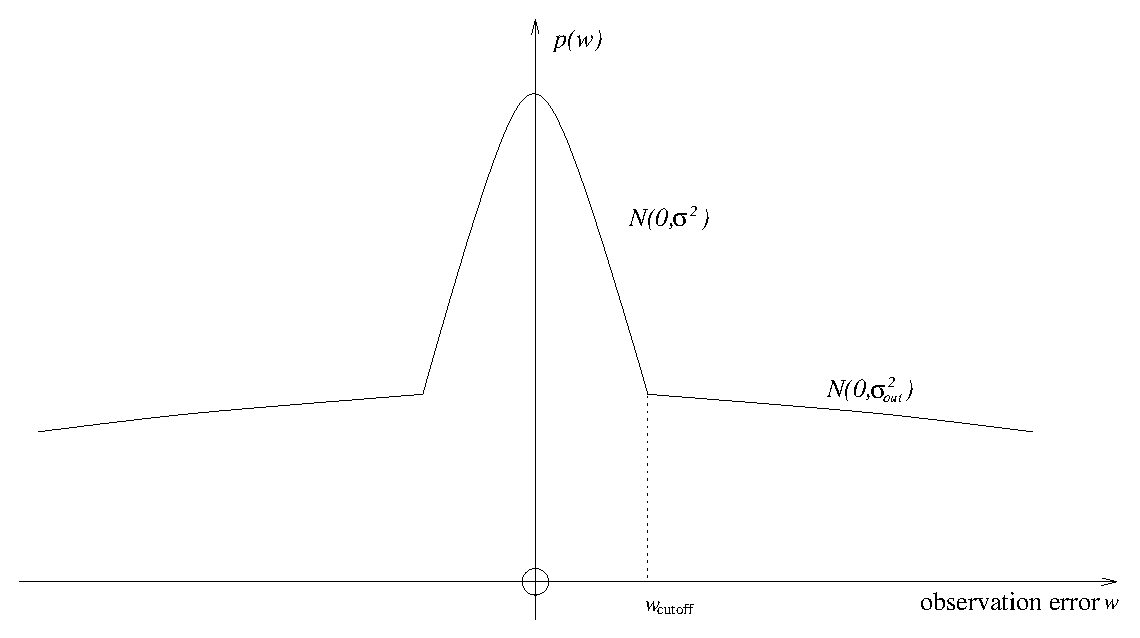
\psfig{file=gauss_mix.ps,width=120mm}}
  \caption{The error model used to model outliers in the observations
	incorporated in robust Levenberg-Marquardt,
	a combination of a narrow inlier Gaussian with
	variance $\sigma^2$, and wide Gaussian for outliers with
	variance $\sigma_{\rm out}^2$. Both distributions on the
	observation error $w$ have zero mean.}
 \label{gauss_mix}
\end{figure}
The distribution is a function of the observation error\footnote{The innovation
$\nuvec$ is the observation error relative to that computed from the
{\em estimated} state: $\nuvec = \zvec - \hvec(\xhat)$.}
$\wvec = \zvec - \hvec(\xvec)$.
The relative vertical scaling of the two Gaussians is chosen so that the
two distribution functions are equal at a chosen point $x_{\rm offset}$.

For a general multi-dimensional observation, we have a inverse covariance
matrix $N\inv$ for the inlier distribution.
We restrict the outlier distribution $N_{\rm out}\inv$ to be a rescaled version
of the inlier distribution, so that
\[ N_{\rm out}\inv = \frac{1}{V} N\inv
\]
for some value $V>1$. We then set choose a cutoff hypersphere in the state
space $\xvec$ for switching between the two distributions as a particular
value of the $\chi^2$. So the probability distribution function is
\[ p(\nuvec) = \left\{ \begin{array}{ll} e^{-\nuvec\tr N\inv \nuvec} &
    \mbox{if}\;\;\;\nuvec\tr N\inv \nuvec < \chi_{\rm cutoff}^2\;\;\mbox{(inlier)} \\&\\
		 e^{K\inv -1} e^{-\nuvec\tr N_{\rm out}\inv \nuvec}
  & \mbox{otherwise (outlier)} \end{array} \right.
\]
The scaling of the outlier distribution is chosen so that the two distributions
are correctly aligned at the chosen cutoff point $\chi_{\rm cutoff}^2$.
This leads directly to the correct ``compensation'' value for the likelihood
function $1-K\inv\chi_{\rm cutoff}^2$, to be added to the least-squares
residual when the outlier distribution is selected during application
of a minimisation iteration.
The simple scheme used to decide switching between the
two distributions is detailed below.
Note that each Levenberg-Marquardt observation can be chosen as robust
or standard (non-robust), and potentially with a different choice for
$K$ and $\chi_{\rm cutoff}^2$.

\subsection{Generalised observations}
The observation function $\hvec(.)$ in Equation~\ref{measure_equation}
does not encapsulate the most general
form of observation, since it assumes that the observation vector $\zvec$
can be separated as a function of the state $\xvec$. It is sometimes therefore
necessary to introduce a generalised observation of the form
\[ \Fvec(\xvec,\zvec-\wvec) = \vecz
\]
where $\wvec$ again represents a random noise vector having covariance $N$.
However with some manipulation and extra computation we can effectively
convert the linearised version of the $\Fvec$-type function into an
$\hvec$-type function, allowing it to be incorporated in the same way.
We linearise $\Fvec(.)$ with respect to $\xvec$ and $\zvec$ around the
estimated state $\xhat$ and observation $\zvec$, assuming
that the noise $\wvec$ is small:
\[ \Fvec(\xvec,\zvec_t) = \Fvec(\xhat,\zvec)
	+ \frac{\partial \Fvec}{\partial \xvec} (\xvec-\xhat)
	- \frac{\partial \Fvec}{\partial \zvec} \wvec = \vecz
\]
where $\xvec$ here represents the true value of the state vector, and $\zvec_t$
is the true observation vector (as opposed to the actually measured vector
$\zvec$), so that $\wvec = \zvec-\zvec_t$.
We identify the following quantities with their equivalents for an $\hvec$-type
observation:
\begin{description}
  \item{The {\bf innovation}} vector is $\nuvec=-\Fvec(\xhat,\zvec)$.
  \item{The {\bf Jacobian}} matrix is
	$H=\frac{\partial \Fvec}{\partial \xvec}$.
  \item{The {\bf noise vector}} is
	$\wvec' = \frac{\partial \Fvec}{\partial \zvec} \wvec$.
  \item{The {\bf noise covariance}} matrix is
	$N' = \frac{\partial \Fvec}{\partial \zvec} N \left(\frac{\partial \Fvec}{\partial \zvec}\right)\tr$.
\end{description}
Extra computation is therefore needed to convert the observation covariance
from $N$ to $N'$. The innovation vector $\nuvec$, Jacobian matrix $H$ and
observation covariance $N'$ are substituted into the Levenberg-Marquardt
algorithm in place of their equivalents for the $\hvec$-type observation.
There is no reason why there should not be a robust version of the $\Fvec$-type
observation, but currently it is not implemented.

\subsection{Levenberg-Marquardt software}
The following code extracts are taken from the {\tt vision/vision\_test.c}
test program. The example application is fitting a quadratic function through
points $x,y$ on a plane. The function to be fitted is
\[ y = ax^2 + bx + c
\]
The state vector of unknown parameters to be estimated is thus
\[ \xvec = \beginm{c} a \\ b \\ c \endm
\]
and we wish to compute the least-squares solution that minimises
\[ J(\xvec) = \sumjk (y_j - ax_j^2 - bx_j - c)^2 \sigma_j^{-2}
\]
given $k$ points $x_j,y_j$ for  $j=1,\ldots,k$ and independent noise
levels $\sigma_j$ for each point $j$. This can be solved directly by
linear methods, and this feature makes it useful as a test algorithm because
test program can compare the results with the Levenberg-Marquardt solution.
The problem can be put into the form of the Levenberg-Marquardt algorithm
described above by identifying
\[ \zvec\brj = (y_j),\;\;\;N\inv\brj = (\sigma^{-2}),\;\;\;
   \hvec(\xvec) = ax_j^2 + bx_j + c
\]

To initialise a Levenberg-Marquardt algorithm instance use the call
\begin{verbatim}
      Gan_LevMarqStruct *lm;

      /* initialise Levenberg-Marquardt algorithm */
      lm = gan_lev_marq_alloc();
\end{verbatim}
We build the points from ground-truth values for the quadratic coefficients
$a,b,c$, and add random Gaussian noise:
\begin{verbatim}
      /* number of points */
      #define NPOINTS 100

      /* ground-truth quadratic coefficients a,b,c */
      #define A_TRUE 2.0
      #define B_TRUE 3.0
      #define C_TRUE 4.0

      /* noise standard deviation */
      #define SIGMA 1.0

      /* arrays of x & y coordinates */
      double xcoord[NPOINTS], ycoord[NPOINTS];

      /* build arrays of x & y coordinates */
      for ( i = NPOINTS-1; i >= 0; i-- )
      {
         /* x-coordinates evenly spaced */
         xcoord[i] = (double) i;

         /* construct y = a*x^2 + b*y + c + w with added Gaussian noise w */
         ycoord[i] = A_TRUE*xcoord[i]*xcoord[i] + B_TRUE*xcoord[i]
                     + C_TRUE + gan_normal_sample(0.0, SIGMA);
      }
\end{verbatim}
Here we defined a noise level {\tt SIGMA} as the estimated standard deviation
of the random observation errors, the same for each point.
Now that we have constructed the input data, the next thing is to create
observations for each point.
Gandalf's version of Levenberg-Marquardt uses callback functions to
evaluate observation $\hvec(.)$ and observation Jacobians $H$.
A non-robust h-type observation is then defined by:
\begin{itemize}
  \item The observation vector $\zvec$;
  \item The observation inverse covariance $N\inv$, and;
  \item The observation callback function $\hvec(.)$.
\end{itemize}
We construct the observations for the quadratic fitting problem using the
following code:
\begin{verbatim}
      Gan_Vector *z; /* define observation vector */
      Gan_SquMatrix *Ni; /* define observation inverse covariance */

      /* allocate observation vector z and inverse covariance Ni */
      z = gan_vec_alloc(1);
      Ni = gan_symmat_fill_va ( NULL, 1, 1.0/(SIGMA*SIGMA) );

      for ( i = NPOINTS-1; i >= 0; i-- )
      {
         /* construct point observation */
         z = gan_vec_fill_va ( z, 1, ycoord[i] );
         cu_assert ( z != NULL );
         cu_assert ( gan_lev_marq_obs_h ( lm, z, &xcoord[i], Ni, quadratic_h )
                     != NULL );
      }
\end{verbatim}
We create the observation vector with size one; this can be adjusted
dynamically if necessary; see Section~\ref{set-size-vec-sec}.

The observation callback function {\tt quadratic\_h()} is defined as follows:
\begin{verbatim}
      /* observation callback function for single point */
      static Gan_Bool
       quadratic_h ( Gan_Vector *x,  /* state vector */
                     Gan_Vector *z,  /* observation vector */
                     void *zdata,    /* user pointer attached to z */
                     Gan_Vector *h,  /* vector h(x) to be evaluated */
                     Gan_Matrix *H ) /* matrix dh/dx to be evaulated or NULL */
      {
         double a, b, c;

         /* read x-coordinate from user-defined data pointer */
         double xj = *((double *) zdata);

         /* read quadratic parameters from state vector x=(a b c)^T*/
         if ( !gan_vec_read_va ( x, 3, &a, &b, &c ) )
         {
            gan_err_register ( "quadratic_h", GAN_ERROR_FAILURE, NULL );
            return GAN_FALSE;
         }

         /* evaluate h(x) = h(a,b,c) = y = a*x*x + b*x + c */
         if ( gan_vec_fill_va ( h, 1, a*xj*xj + b*xj + c ) == NULL )
         {
            gan_err_register ( "quadratic_h", GAN_ERROR_FAILURE, NULL );
            return GAN_FALSE;
         }

         /* if Jacobian matrix is passed as non-NULL, fill it with the Jacobian
            matrix (dh/da dh/db dh/dc) = (x*x x 1) */
         if ( H != NULL &&
              gan_mat_fill_va ( H, 1, 3, xj*xj, xj, 1.0 ) == NULL )
         {
            gan_err_register ( "quadratic_h", GAN_ERROR_FAILURE, NULL );
            return GAN_FALSE;
         }

         /* success */
         return GAN_TRUE;
      }
\end{verbatim}
Note the the $x$-coordinate passed in as the third ``user pointer'' argument
to {\tt gan\_lev\_marq\_obs\_h()} is read into the variable {\tt xj} in
{\tt quadratic\_h()}. Using pointers in this way is the standard method
to pass extra information into the callback routines.

So far we have merely registered the observations and their callback
routines. No processing has started. To get started with some actual
optimisation we need to initialise the state vector with some values for
$a$, $b$ and $c$. This involves invoking the routine
\begin{verbatim}
      double residual;

      /* initialise Levenberg-Marquardt algorithm */
      gan_lev_marq_init ( lm, quadratic_init, NULL, &residual );
\end{verbatim}
{\tt quadratic\_init()} is another callback routine that computes values for
the state vector $\xvec$ given the observations $\zvec\brj$. The observations
are presented to {\tt quadratic\_init()} in a linked list. The third argument
to {\tt gan\_lev\_marq\_init()} is another user pointer, not used in this
example. The last {\tt residual} argument is returned as the initial
value of the least-squares residual $J(\xvec)$. This is the full code for
the {\tt quadratic\_init()} function, whose operation is self-explanatory:
\begin{verbatim}
      /* initialisation function for state vector */
      static Gan_Bool
       quadratic_init ( Gan_Vector *x0,     /* state vector to be initialised */
                        Gan_List *obs_list, /* list of observations */
                        void *data )        /* user data pointer */
      {
         int list_size = gan_list_get_size(obs_list);
         Gan_LevMarqObs *obs;
         Gan_Matrix33 A;
         Gan_Vector3 b;
         double xj, y;

         /* we need at least three points to fit a quadratic */
         if ( list_size < 3 ) return GAN_FALSE;

         /* initialise quadratic by interpolating three points: the first, middle and
            last point in the list of point observations. We construct equations
      
               (y1)   (x1*x1 x1 1) (a)
               (y2) = (x2*x2 x2 1) (b) = A * b for 3x3 matrix A and 3-vector b
               (y3)   (x3*x3 x3 1) (c)

            and solve the equations by direct matrix inversion (not pretty...) to
            obtain our first estimate of a, b, c given points (x1,y1), (x2,y2) and
            (x3,y3).
         */

         /* first point */
         gan_list_goto_pos ( obs_list, 0 );
         obs = gan_list_get_current ( obs_list, Gan_LevMarqObs );
         xj = *((double *) obs->details.h.zdata); /* read x-coordinate */
         A.xx = xj*xj; A.xy = xj; A.xz = 1.0; /* fill first row of equations in A */
         gan_vec_read_va ( &obs->details.h.z, 1, &y );
         b.x = y; /* fill first entry in b vector */
    
         /* middle point */
         gan_list_goto_pos ( obs_list, list_size/2 );
         obs = gan_list_get_current ( obs_list, Gan_LevMarqObs );
         xj = *((double *) obs->details.h.zdata); /* read x-coordinate */
         A.yx = xj*xj; A.yy = xj; A.yz = 1.0; /* fill first row of equations in A */
         gan_vec_read_va ( &obs->details.h.z, 1, &y );
         b.y = y; /* fill second entry in b vector */
    
         /* last point */
         gan_list_goto_pos ( obs_list, list_size-1 );
         obs = gan_list_get_current ( obs_list, Gan_LevMarqObs );
         xj = *((double *) obs->details.h.zdata); /* read x-coordinate */
         A.zx = xj*xj; A.zy = xj; A.zz = 1.0; /* fill first row of equations in A */
         gan_vec_read_va ( &obs->details.h.z, 1, &y );
         b.z = y; /* fill second entry in b vector */

         /* invert matrix and solve (don't do this at home) */
         A = gan_mat33_invert_s(&A);
         b = gan_mat33_multv3_s ( &A, &b );

         /* fill state vector x0 with our initial values for a,b,c */
         gan_vec_fill_va ( x0, 3, b.x, b.y, b.z );
         return GAN_TRUE;
      }
\end{verbatim}
We are now ready to apply optimisation iterations using the routine
{\tt gan\_lev\_marq\_iteration()}. The following code
applies ten iterations, adjusting the damping factor in the way suggested
in~\cite{Press:etal:88}. This simple scheme decreases the damping when the
residual decreases, and vice versa.
\begin{verbatim}
      double lambda = 0.1; /* damping factor */
      double new_residual;

      /* apply iterations */
      for ( i = 0; i < 10; i++ )
      {
         gan_lev_marq_iteration ( lm, lambda, &new_residual );
         if ( new_residual < residual )
         {
            /* iteration succeeded in reducing the residual */
            lambda /= 10.0;
            residual = new_residual;
         }
         else
            /* iteration failed to reduce the residual */
            lambda *= 10.0;
      }
\end{verbatim}
To extract the optimised solution, use the code
\begin{verbatim}
   Gan_Vector *x;

   /* get optimised solution */
   x = gan_lev_marq_get_x ( lm );
\end{verbatim}
Note that the {\tt x} pointer passed back here points to a vector internal
to the Levenberg-Marquardt software, and should {\em not} be freed.
To free the Levenberg-Marquardt structure and the matrices \& vectors
created above, use the code
\begin{verbatim}
   gan_squmat_free ( Ni );
   gan_vec_free ( z );
   gan_lev_marq_free ( lm );
\end{verbatim}

\section{Fast Hough Transform}
\begin{verbatim}
      #include <gandalf/vision/fast_hough_transform.h>
\end{verbatim}
A Hough transform is a mapping from an {\em observation space} into a
{\em parameter space}. In computer vision, observation space could be a
digital image, an edge map etc. Now assume that
a certain structure is thought to be present in image space. For an edge
map, this could be a straight line or a circle. The parameters of the
structure define parameter space (gradient and intercept for a line, radius
and centre coordinates for a circle). In a Hough transform, each point
in image space ``votes'' for that part of parameter space which describes
structures which include the point. For instance, to find circles in an
edge map, edges vote for the region in parameter space (in fact a conical
surface) which describes circles that pass through them. A part of parameter
space receiving a large number of votes corresponds to a possible fit.

In the normal Hough transform approach, parameter space is bounded by
setting lower and upper limits on the parameter values, and then divided
into blocks in each direction, and an accumulator assigned
to each block. The Hough transform proceeds with each point in image space
being transformed to an region in parameter space as described in the
previous paragraph. When the region intersects one of the blocks,
the corresponding accumulator is incremented. The block whose
accumulator has the most
votes can then be taken as the best fit of the structure to the image
points, the values of the parameters usually being calculated at the
centre of the block.

%Figure~\ref{Hough_example} illustrates the Hough transform
%in action in an actual problem, that of fitting a straight line to points
%on a plane.
%\begin{figure}
%  \vspace{7.5in}
%  \caption[Application of the Hough transform to line fitting.]
%	   {Application of the Hough transform to line fitting. a) Points on
%	    a plane. b) Result of Hough transform. c) Number of votes for
%	    each block in parameter space. d) Best fit line superimposed on
%	    original points.}
%   \label{Hough_example}
%\end{figure}
%If the plane has coordinates $(u,v)$ the line can be written
%\begin{equation}
%   v=\alpha u + \beta
%   \label{line_hough_eq}
%\end{equation}
%where $\alpha$ and $\beta$ are constant. Parameter space is hence
%$(\alpha,\beta)$. In figure~\ref{Hough_example}a
%twenty points are placed on a line with gradient $\alpha =-0.5$ and
%intercept $\beta = 1$ and a small amount of Gaussian distributed error
%is added (standard deviation 0.5). Sixty
%randomly positioned points are added. All the points lie in the square on
%the $(u,v)$ plane defined by $-5<u<5$, $-5<v<5$.
%The region of parameter space voted for by each point $(u,v)$ can
%be obtained by rearranging equation~\ref{line_hough_eq} above:
%\begin{displaymath}
%   \beta = -u \alpha + v.
%\end{displaymath}
%This is a straight line in parameter space $(\alpha,\beta)$ with gradient
%$-u$ and intercept $v$. Points on this line describe lines in image space
%passing through the point $(u,v)$. Figure~\ref{Hough_example}b shows the
%points $(u,v)$ transformed into the lines in parameter space they vote for.
%The parameters are then restricted to the range $-5<\alpha<5$,
%$-10<\beta<10$.
%The grid superimposed on figure~\ref{Hough_example}b is the division of
%this restriction of parameter space into equally sized blocks, 32 blocks
%in both the $\alpha$ and $\beta$ directions. Figure~\ref{Hough_example}c
%shows the number of votes received by each block, i.e. the number of lines
%intersecting with each block. The block with the highest number of votes,
%26, is shown in bold. Since this number is greater than 20, several noise
%points were close enough to the line to vote for the best fit line by chance.
%At the centre of the winning block the values of $\alpha$ and
%$\beta$ are -0.46875 and 0.9375 respectively, and the corresponding line
%is shown with the original points in figure~\ref{Hough_example}d.

\subsection{The Fast Hough Transform (FHT)}
\label{FHT_section}
The above method has two main drawbacks: large memory requirement and
slowness. In order to find the plane parameters accurately, parameter space
must be divided finely in all three directions, and an accumulator assigned
to each block. Also it takes a long time to fill the accumulators when
there are so many. The Fast Hough Transform described in~\cite{Li_etc_86}
gives considerable speed up and reduces memory
requirement. Instead of dividing parameter space uniformly into blocks,
the FHT ``homes in'' on the solution, ignoring areas in parameter space
relatively devoid of votes. The relative speed advantage of the FHT
increases for higher dimensional parameter spaces.

The FHT applies to those Hough transform problems in which a feature
$F_j$ votes for a {\em hyperplane} in parameter space (a hyperplane is
a $k-1$ dimensional generalisation of a plane, where $k$ is the dimension
of parameter space). This means that the relationship between feature space
and parameter space must be linear in the parameters.
In addition, it must be known in
advance how many votes the solution will receive in the Hough
transform.
% In the example shown in figure~\ref{Hough_example} above,
%this means that it must be known in advance that there are about
%twenty points on the line, in order for the FHT to be used.
%This is because of a threshold $T$ that is fundamental to the algorithm.
The FHT is also restricted in that it only supplies one
``best fit'' solution, whereas for the more conventional Hough transform
method above it is plausible to consider local maxima as alternatives to
the global maximum, i.e. the block in parameter space
receiving the most votes.

A major advantage of the FHT is that it only uses addition and
multiplication by two, which in integer arithmetic can be done
efficiently using bitwise shifts. This is very convenient for computers
on which integer arithmetic is much faster than floating point arithmetic.

\subsubsection{Notation}
 The following notation is taken from~\cite{Li_etc_86}.
 Hyperplanes are represented by the equations
 \begin{equation}
     \label{hyperpln_eq}
     a_{0j} + \sum_{i=1}^k a_{ij} X_i = 0\;\;\;{\rm for} ~j~=~1,2,\ldots,n
 \end{equation}
 where $(X_1,X_2,\ldots, X_k)$ is parameter space, rescaled so that
 the initial ranges of each $X_i$ are the same and centred around zero.
 The initial ranges thus
 form a {\em hypercube} (generalisation of a cube) in parameter space. Each
 $a_{ij}$ is a function of $F_j$  normalised such that
 $\sum_{i~=~1}^k a_{ij}^2 = 1$.

\subsubsection{The FHT Algorithm} \label{FHT_alg}
 A coarse Hough Transform is applied to the initial ``root'' hypercube in
 parameter space by dividing it into $2^k$ ``child''
 hypercubes formed by halving the root along each of the $k$ dimensions and
 assigning an accumulator to each child. Each hyperplane passing through
 a child hypercube increments its accumulator. Those children receiving
 greater than a threshold $T$ votes are recursively subdivided, becoming
 parents themselves, and so on.

 A limit is set on the level of subdivision. Because the range of the
 parameters in a hypercube is halved for each level of subdivision,
 This is equivalent to having a precision threshold:
 \begin{displaymath}
     {\rm maximum\;subdivision\;level}=\log_2
      {\rm \frac{initial\;range}{required\;accuracy}}.
 \end{displaymath}

 An extra speed up is made possible by keeping track of which features vote
 for (i.e. which hyperplanes intersect) each hypercube.
 Only those features need be tested for intersection
 between hyperplane and child hypercubes, since children lie inside their
 ``parents''.

 Li et al. consider two methods of calculating whether a hyperplane passes
 through a hypercube. The ``brute force'' method is to test whether all
 the vertices of the hypercube are on the same side of the hyperplane by
 evaluating the left hand side of equation~\ref{hyperpln_eq} for each
 vertex. For increased speed, Li et al. recommend determining whether the
 hyperplane intersects the hypercube's circumscribing hypersphere.
 This is an approximation, since some planes will intersect the
 hypersphere but not the hypercube. One effect of this is that the
 total number of subdivisions will be increased, because a hypersphere
 may get more than $T$ votes when the hypercube on its own
 (being smaller) would not have. However the increased speed more
 than compensates for this, especially for high-dimensional
 parameter spaces. The method is fast because the perpendicular distance
 from the centre of a child hypercube to a hyperplane can be
 calculated simply in terms of the corresponding distance from the parent's
 centre to the hyperplane, as is shown on page~\pageref{lookup_table}.
 This distance is then compared with the radius of the hypersphere.

\subsubsection{Example: Line Fitting} \label{line_fitting}
 Figure~\ref{hypercircle}
% and~\ref{FHT_k=2}
 shows how the FHT works for $k=2$, when parameter space is a plane,
 hyperplanes are straight lines and hypercubes are squares whose associated
 hyperspheres are circles passing through the vertices of the squares
 (figure~\ref{hypercircle}).
 \begin{figure}
     \centerline{\psfig{file=hyper.ps,width=100mm}}
     \caption[Calculating the intersection between hyperplanes and
	      hyperspheres.]
	     {This illustrates the approximate method of calculating
	      intersections between hyperplane and hypercube in the Fast Hough
	      Transform in the case $k=2$. A line is tested for intersection
	      with the square's circumscribing circle rather than the square
	      itself. This method give the same result for lines like $A$ and
	      $B$, but not for line $C$}
     \label{hypercircle}
 \end{figure}
 This is applicable to the
 problem of finding a straight line through points on a plane. If the
 plane has coordinates $(u,v)$ the line can be written
 \begin{displaymath}
   v=\alpha u + \beta
 \end{displaymath}
 where $\alpha$ and $\beta$ are constant. Each point
 $(u_j , v_j )$ votes for a line in parameter space:
 \begin{displaymath}
     \beta=v_j - \alpha u_j .
 \end{displaymath}
 Let the initial ranges of $\alpha$ and $\beta$, defining the root
 hypercube, be $L_{\alpha}$ and
 $L_{\beta}$ centred around $\alpha_0$ and $\beta_0$ respectively.
 Then the above equation can put in the form of
 equation~\ref{hyperpln_eq} using the transformation
 \begin{displaymath}
     X_1 = \frac{\alpha}{L_\alpha} ,\;
     X_2 = \frac{\beta}{L_\beta} ,\;
     a_{0j} = \frac{- v_j}{q} ,\;
     a_{1j} = \frac{L_\alpha u_j}{q} ,\;
     a_{2j} = \frac{L_\beta}{q}
 \end{displaymath}
 where $q = \sqrt{L_\alpha^2 u_j^2 + L_\beta^2}$.

% Figure~\ref{FHT_k=2} illustrates the FHT line finder applied to the
% data already used above to illustrate the conventional Hough transform.
% \begin{figure}
%     \centerline{\psfig{file=linefitting.ps,width=80mm}}
%     \caption[Application of the Fast Hough transform to line fitting.]
%	     {Application of the Fast Hough transform to line fitting.
%	      a) Points on a plane. b) The FHT recursive subdivision of
%	      parameter space. c) Winning block with the lines that voted
%	      for it. d) Best fit line with the points that voted for it
%	      (thick crosses).}
%     \label{FHT_k=2}
% \end{figure}
% The eighty points are shown in figure~\ref{FHT_k=2}a. The threshold $T$
% is set to 20, and the limit on the level of subdivision set to 5.
% The initial ranges of $\alpha$ and $\beta$ are again chosen as
% $-5<\alpha<5$, $-10<\beta<10$. This root rectangle (or square in
% $(X_1 , X_2 )$ space) is recursively subdivided, with rectangles
% subdivided if they receive greater than 20 votes. Figure~\ref{FHT_k=2}b
% shows the FHT ``homing in'' on the solution.
% The best fit line is identical to that found previously, i.e.
% $\alpha=-0.46875$, $\beta=0.9375$. 27 points voted for this line, i.e. one
% more than previously, the extra vote coming from a Hough transformed
% line intersecting a block's circumscribing circle but missing the block
% itself. The FHT keeps track of which lines pass through which circles,
% and the lines that voted for the winning block are shown
% in figure~\ref{FHT_k=2}c.
% The points to which they correspond are displayed in
% figure~\ref{FHT_k=2}d along with the best fit line.

\subsection{Example: Plane Fitting} \label{plane_fit_sec}
 The method described here was used in~\cite{McLauchlan_91}.
 A pair of images is rectified so that their epipolar lines are
 horizontal and parallel. Edges are detected in each image.
 A region of the left image is then matched to the right image
 using a planar fit in $(x,y,d)$ space where $(x,y)$ are
 the coordinates of edges in the left image and $d$ is the disparity,
 such that if $(x_r,y_r)$ are the coordinates of the corresponding edge
 in the right image,
 \[ x_r = x + d \]
 and because of the rectification procedure, $y_r=y$.
 
 A planar fit is attempted to the disparity points from candidate
 edge matches between the image, in the knowledge that planes in
 disparity space $(x,y,d)$ correspond to planes in the world.

 A large number of the disparity points in the box will be
 incorrect matches, so direct fitting, for example for least squares, would
 not work. However the Hough transform is well suited to such a problem.
 It is used to select a large subset of the disparity points that lie
 near a plane. The Fast Hough transform
 gives a large increase in speed and decrease in storage
 requirement over the standard Hough transform method.
 It is applicable because, with an appropriate parametrisation,
 plane fitting is a linear Hough transform problem, to which the FHT
 is restricted.

 \subsubsection{Calculating the Intersection of a Plane and a Sphere}
  The perpendicular, and therefore nearest, distance from the plane to the
  centre of the cube is calculated. If it is smaller than the radius
  of the circumscribing sphere, the plane intersects the sphere,
  otherwise it misses. The distance is normalised by dividing it by
  the side length of the cube. The normalised distance of a plane
  from the centre of a child cube can be calculated simply from the
  normalised distance of the plane from it's parent's centre, as shown below.
  The plane is defined by the following equation:
  \begin{displaymath}
     a_0 + a_1 X_1 + a_2 X_2 + a_3 X_3 = 0
  \end{displaymath}
  where $a_1^2 + a_2^2 + a_3^2 = 1$. Let the child cube have indices
  $[b_1, b_2, b_3]$, centre $(C_1,C_2,C_3)$ and side length $L_{\rm child}$.
  The radius of the circumscribing sphere is
  $\frac{\sqrt{3} L_{\rm child}}{2}$. The perpendicular distance
  of the plane to the centre of the child cube is
  \begin{eqnarray}
     \rm{perpendicular\;distance} & = &
      \frac{a_0 + a_1 C_1 + a_2 C_2 + a_3 C_3}{\sqrt{a_1^2 + a_2^2 + a_3^2}}
      \nonumber \\
     & = & a_0 + a_1 C_1 + a_2 C_2 + a_3 C_3. \nonumber
  \end{eqnarray}
  When normalised this becomes
  \begin{equation}
     \label{child_norm_dist}
     R_{\rm child} = \frac{a_0 + a_1 C_1 + a_2 C_2 + a_3 C_3}{L_{\rm child}}.
  \end{equation}
  The normalised distance of the centre of the parent from the plane,
  where the parent has centre $(p_1,p_2,p_3)$ and side length
  $L_{\rm parent}$, is
  \begin{displaymath}
     R_{\rm parent} = \frac{a_0 + a_1 p_1 + a_2 p_2 + a_3 p_3}{L_{\rm parent}}.
  \end{displaymath}
  The child is half the size of the parent, so
  $L_{\rm parent} = 2 L_{\rm child}$. Also the centres of the cubes are
  related by the following equation:
  \begin{equation}
     \label{pc_centres}
     C_i = p_i + \frac{b_i L_{\rm child}}{2}.
  \end{equation}
  and substituting the RHS into equation~\ref{child_norm_dist} yields
  \begin{eqnarray}
     R_{\rm child} & = & \frac{a_0 + a_1 p_1 + a_2 p_2 + a_3 p_3 +
		               \frac{L_{\rm child}}{2}
			       (a_1 b_1 + a_2 b_2 + a_3 b_3)}
			      {L_{\rm child}} \nonumber \\
     & = & 2 R_{\rm parent} + \frac{1}{2} (a_1 b_1 + a_2 b_2 + a_3 b_3) .
	\label{recurs_dist}
  \end{eqnarray}
  This \label{lookup_table} formula is used to calculate the normalised
  distance for a child in terms of that of it's parent, and is fast because
  the $2^k$ values of the term
  $\frac{1}{2} (a_1 b_1 + a_2 b_2 + a_3 b_3)$ can be stored as a look-up
  table for each set of coefficients $a_{ij}$ (i.e. each disparity point).

  The normalised distance of the plane from the root cube, which has side
  length one and centre $(0,0, \frac{d_{\rm peak}}{w})$, is
  \begin{equation}
     R_{\rm root} = a_0 + a_3 \frac{d_{\rm peak}}{w}.
     \label{root_distance}
  \end{equation}
  The normalised distances are calculated initially
  from equation~\ref{root_distance} and from
  then on using the formula~\ref{recurs_dist}.
  The normalised distances are compared with $\frac{\sqrt{3}}{2}$,
  the radius of the circumscribing sphere of a cube with side length one.
  This is equivalent to comparing the un-normalised distance with the
  circumscribing sphere of the original cube.

 \subsubsection{Calculating the Plane Parameters of a Child Cube}
  When a new ``best so far'' fit cube is found,
  the cube needs to find out where it is in parameter space.
  The FHT does not explicitly propagate information from parent to child
  concerning the position of hypercubes in parameter space.
  Of course it
  would be trivial to do this, by, for instance, calculating the centre
  of the child relative to the centre of the parent,
  using equation~\ref{pc_centres}, and passing
  the centre coordinates on to the child.
  However, since centre coordinates are needed {\em only} when an
  improved planar fit is found, this would involve quite a lot of wasted
  multiplication and division.

  The method used in Needles provides each cube with the part of its
  ``family tree'' comprising the direct line of descent from the root
  to itself. It therefore knows how it is related to its parent, how
  its parent was related to its grandparent, and so on. A cube knows
  only about its own ``branch'', which is passed down to it by its parent.

  The relationship between parent and child cubes is contained in the
  child indices $[b_1, b_2, b_3]$.
  Each cube therefore receives a list of such index triplets, detailing
  the relationships between ancestors of different generations.
  The list is linked {\em backwards}, i.e. from child to root. The formulae
  to calculate a cube's centre coordinates are simpler when the list
  is traversed in this direction. They are computational in nature,
  involving iteration when traversing the list, so we have not included
  them here, but they are given in the next section in procedure
  $cube\_centre$.
 \subsubsection{Formal Statement of the FHT Plane Fitting Algorithm}
  \label{formal_FHT}
  We have:
  \begin{enumerate}
     \item A set of disparity points $(x_j , y_j , d_j )$, $j=1 \ldots n$.

     \item An array of weights $W_j$, $j=1 \ldots n$, one for each
	   disparity point $(x_j , y_j , d_j )$.

     \item Parameter space $(a,b,c)$, restricted to the box with centre
	   $(0,0,d_{\rm centre})$ and side lengths $L_a$, $L_b$ and $L_c$.
	   $d_{\rm centre}$ is the centre of the disparity search range.

     \item A vote threshold $T= \theta W$, $W$ being the total weight of
	   the edges in the square patch.

     \item A minimum level of subdivision $l_{\min}$ (e.g. 3), and a
	   maximum level $l_{\max}$ (e.g. 10).
  \end{enumerate}
  The algorithm is as follows:

  {\bf begin}
  \begin{indent_para}
     Declare new variables:
     \begin{indent_para}
      An array ${\bf R}$ of distances $R_j$, $j=1 \ldots n$.

      An array ${\bf P}$ of boolean flags $P_1, P_2,\ldots,P_n$ where each
      $P_j$ either takes the value $true$ or $false$.

      Integer variables $max\_level$ and $max\_value$, initialised to zero.

      Variables $a_{\rm best}$, $b_{\rm best}$ and $c_{\rm best}$
      making up a point in $(a,b,c)$ space.

      Another array of boolean flags ${\bf P}_{\rm best}$.
     \end{indent_para}

     The variables $max\_level$, $max\_value$, $a_{\rm best}$, $b_{\rm best}$,
     $c_{\rm best}$ and array ${\bf P}_{\rm best}$ are used to keep track
     of the best fit as the algorithm proceeds.

     Set all the $P_j$ to $false$.

     For each disparity point $(x_j , y_j , d_j )$:

     {\bf begin}
     \begin{indent_para}
      Calculate the plane parameters for $(X_1 , X_2 , X_3 )$ space:
      \begin{displaymath}
	   a_{0j} = \frac{-d_j}{Q} ,\;
	   a_{1j} = \frac{L_a x_j}{Q} ,\;
	   a_{2j} = \frac{L_b y_j}{Q} ,\;
	   a_{3j} = \frac{L_c}{Q}
      \end{displaymath}
      where $Q = \sqrt{L_a^2 x_j^2 + L_b^2 y_j^2 + L_c^2}$.

      Calculate the normalised perpendicular distance $R_j$
      from the plane to the centre of the root cube:
      \begin{displaymath}
 	   R_j = a_{0j} + \sum_{i=1}^3 a_{ij} C_i
	   = a_{0j} + \frac{a_{3j} d_{\rm centre}}{Q L_c}.
      \end{displaymath}

      If $R_j < \frac{\sqrt{3}}{2}$ the plane passes through
      the root cube's circumscribing sphere: set $P_j$ to $true$.
     \end{indent_para}
     {\bf end}

     Call the procedure $divide\_cube$ with arguments as follows:
     \begin{enumerate}
            \item Array of boolean flags ${\bf P}$.

	    \item Array ${\bf R}$ of normalised distances.

	    \item Initial level of subdivision 0.

	    \item Initial accumulator value 0.

	    \item Empty line of descent list.
     \end{enumerate}
  \end{indent_para}
  {\bf end}

  Procedure $divide\_cube$ ( array of flags ${\bf P}$, array of normalised
  distances ${\bf R}$, subdivision level $l$,
  accumulator value $v$, line of descent list ):

  {\bf begin}
  \begin{indent_para}
     Declare new variables:
     \begin{indent_para}
      Eight boolean flags arrays ${\bf P}_{\bf b}$, one for
      each ${\bf b}$, where ${\bf b}$
      is a child cube index triplet $(b_1 , b_2 , b_3 )$ and each $b_i$ is
      either -1 or 1. All the elements of the flag arrays are initialised
      to $false$.

      Eight arrays ${\bf R}_{\bf b}$ of normalised distances.

      Accumulators $A_{\bf b}$ for each ${\bf b}$, initialised to zero.

      Boolean flag $s$, initialised to $false$.
     \end{indent_para}
     Sum the votes for the child cubes: for each $j$ such that $P_j = true$:

     {\bf begin}
     \begin{indent_para}
      For each child cube with index {\bf b}:

      {\bf begin}
      \begin{indent_para}
       Calculate the normalised distance $R_{j {\bf b}}$ from plane $j$
       to the centre of the child cube:
       \begin{displaymath}
	R_{j {\bf b}} = 2R_j + \frac{1}{2}
	(a_{1j} b_1 + a_{2j} b_2 + a_{3j} b_3).
       \end{displaymath}
       (The $a_{1j} b_1 + a_{2j} b_2 + a_{3j} b_3$ values can be
	efficiently calculated by storing them in eight arrays, one for each
	${\bf b}$.)

       If $R_{j {\bf b}} < \frac{\sqrt{3}}{2}$ then

       {\bf begin}
       \begin{indent_para}
	Add weight $W_j$ to $A_{\bf b}$

	Set flag $P_{j {\bf b}}$ to $true$.
       \end{indent_para}
       {\bf end}
       \end{indent_para}
      {\bf end}
     \end{indent_para}
     {\bf end}

     Subdivide child cubes receiving greater than or equal to $T$ votes:
     If $l < l_{\rm max}$:

     {\bf begin}
     \begin{indent_para}
      For each child cube with index {\bf b}:

      {\bf begin}
      \begin{indent_para}
       If $A_{\bf b} \geq T$ recursively subdivide child cube:

       {\bf begin}
       \begin{indent_para}
	Add ${\bf b}$ to original line of descent.

        Call $divide\_cube$ with arguments ${\bf P}_{\bf b}$,
	${\bf R}_{\bf b}$, $l+1$, $A_{\bf b}$ and extended line of descent.

	Set flag $s$ to $true$.
       \end{indent_para}
       {\bf end}
      \end{indent_para}
      {\bf end}
     \end{indent_para}
     {\bf end}

     If $s$ is still $false$ (i.e. no further
     subdivision of this cube), test for best fit so far:

     \begin{indent_para}
      If $l > max\_level$ or if $l = max\_level$ and $v > max\_value$:

      {\bf begin}
      \begin{indent_para}
       Set $max\_level$ to $l$.

       Set $max\_value$ to $v$.

       Calculate centre of cube in $(a,b,c)$ space by calling procedure
       $cube\_centre$ with the line of descent as argument. The results are
       copied into $a_{\rm best}$, $b_{\rm best}$ and $c_{\rm best}$.

       Copy array of flags ${\bf P}$ into array ${\bf P}_{\rm best}$.
      \end{indent_para}
      {\bf end}
     \end{indent_para}
    \end{indent_para}
    {\bf end} (procedure $divide\_cube$)

    Procedure $cube\_centre$ ( line of descent list ):
    {\bf begin}
    \begin{indent_para}
     Declare new variables:
     \begin{indent_para}
      Three arrays ${\bf r}_a$, ${\bf r}_b$ and ${\bf r}_c$, each of three
      elements with indices -1, 0 and 1, so that
      ${\bf r}_a = [r_a(-1),r_a(0),r_a(1)]$ and similarly for ${\bf r}_b$
      and ${\bf r}_c$. The zero (middle) elements of each array are not used.
     \end{indent_para}
     Set arrays ${\bf r}_a$, ${\bf r}_b$ and ${\bf r}_c$ as follows:
     \[
	 \begin{array}{ccc}
	  r_a(-1) = \frac{-L_a}{4}, & r_b(-1) = \frac{-L_b}{4}, &
	  r_c(-1) = \frac{-L_c}{4}, \\
	  r_a(1) = \frac{L_a}{4}, & r_b(1) = \frac{L_b}{4}, &
	  r_c(1) = \frac{L_c}{4}. \\
	 \end{array}
     \]

     Set $a_{\rm best}$, $b_{\rm best}$ and $c_{\rm best}$ to zero.

     While line of descent not traversed (i.e. root cube not yet reached):

     {\bf begin}
     \begin{indent_para}
      Take next triplet of indices ${\bf b}$ on line of descent.

      Replace old values of $a_{\rm best}$, $b_{\rm best}$ and $c_{\rm best}$:
      \[
	  \begin{array}{c}
	   a_{\rm best} \leftarrow \frac{a_{\rm best}}{2} + r_a(b_1) \\
	   b_{\rm best} \leftarrow \frac{b_{\rm best}}{2} + r_b(b_2) \\
	   c_{\rm best} \leftarrow \frac{c_{\rm best}}{2} + r_c(b_3) \\
	  \end{array}
      \]
     \end{indent_para}
     {\bf end}

     Add centre $c$-coordinate of root cube to $c_{\rm best}$ ($a$ and $b$
     coordinates of root are zero):
     \[ c_{\rm best} \leftarrow c_{\rm best} + d_{\rm centre} \]
    \end{indent_para}
  {\bf end} (procedure $cube\_centre$)

  At the end of the algorithm $max\_level$ is the highest level
  of subdivision
  reached. This must be greater than or equal to $l_{\min}$ for the fit
  to be used. $max\_value$ is the highest accumulator value of a
  cube at subdivision level $max\_level$, the cube has centre
  $(a_{\rm best} , b_{\rm best} , c_{\rm best} )$
  and these are the best fit plane parameters.
  The flags ${\bf P}_{j \rm best}$ are $true$ if the $j$'th disparity
  point voted for the winning cube,
  and those disparity points constitute the subset of all the points which
  best fit a plane, given that the total weight of the points must
  exceed $T$. They and the values of $max\_level$ and $max\_value$ can
  stored for use. More precise estimates of the plane
  parameters can be calculated using orthogonal regression.

\subsection{Speed Improvement to FHT Line Finder} \label{MFHT}
\begin{verbatim}
      #include <gandalf/vision/modified_fht.h>
\end{verbatim}
 The Fast Hough Transform can be used to fit a line to points on a plane.
 However the modification to the FHT described here has proved to be slightly
 faster for the line fitting problem, and it requires less memory.
 It can readily be generalised and is applicable to
 the same class of Hough transform problems as standard FHT.
 However for higher dimensional parameter spaces (e.g. plane fitting)
 standard FHT takes over as the faster method. To simplify the notation
 the modified FHT (referred to henceforth as the MFHT)
 is described for line fitting only.

 The FHT line fitter was described in section~\ref{line_fitting} and the
 notation used there will be followed. Points $(u_j,v_j)$, $j=1 \ldots n$
 are scattered on the $(u,v)$ plane. A straight line in the plane is defined as
 \[ v=\alpha u + \beta \]
 where $\alpha$ and $\beta$ are constant. Each point $(u_j,v_j)$ ``votes''
 for a line in parameter space $(\alpha , \beta )$.
 Ranges for $\alpha$ and $\beta$ are specified, so
 $\alpha_1 \leq \alpha \leq \alpha_2$ and $\beta_1 \leq \beta \leq \beta_2$.
 Like the standard FHT, the MFHT proceeds by dividing this root
 rectangle (hypercube) into four ($2^k$) child rectangles and counting the
 lines (hyperplanes) passing through each child rectangle. If the number of
 such intersections for any child is greater than a threshold $T$, the child
 is subdivided. The MFHT differs in that the circumscribing hypersphere
 (in this case ellipse) approximation is not used.
 Intersections between line and rectangle are calculated exactly.
 Hence there is no need to normalise parameter space in order to
 transform the root rectangle into a square, as is required for standard FHT.

 The line in $(\alpha , \beta )$ space defined by a point $(u_j,v_j)$ is
 \[ \beta = - u \alpha + v. \]
 Intersection between line and rectangle is calculated by comparing the
 $\beta$ coordinate of the vertices of the rectangle with the points
 of intersection between the line and the constant $\alpha$
 sides of the rectangle. This is illustrated in figure~\ref{rect_intersect}.
 \begin{figure}
  \centerline{\psfig{file=intersect.ps,width=110mm}}
  \caption[Deciding whether a line intersects a rectangle.]
	  {Deciding whether a line intersects a rectangle (see text).}
  \label{rect_intersect}
 \end{figure}
 The ranges $[\alpha_{\rm low},\alpha_{\rm high}]$ and
 $[\beta_{\rm low},\beta_{\rm high}]$ define a rectangle in
 $(\alpha , \beta )$ space. Three lines $A$, $B$ and $C$ are shown.
 For each line, the $\beta$ values of the intersection points with the lines
 $\alpha = \alpha_{\rm low}$ and $\alpha = \alpha_{\rm high}$
 (points $A_1$ and $A_2$, $B_1$ and $B_2$, $C_1$ and $C_2$
 in figure~\ref{rect_intersect}) are compared with $\beta_{\rm low}$ and
 $\beta_{\rm high}$. The $\beta$ values can be thought of as intercept values
 of the line with the $\alpha = {\rm constant}$ lines.
 It is clear that line and rectangle miss each other if and only if
 if all four vertices are either below or above (i.e. their $\beta$ values
 are all $<$ or $>$) both intercepts. Obviously this is true for line $B$ but
 false for lines $A$ and $C$.

 In practice it saves repeated computational effort if intersections between
 a parent's four child rectangles and the lines are calculated at the same
 time. Let us assume that enough lines intersect the rectangle in
 figure~\ref{rect_intersect} for it to be subdivided.
 It is divided into four child rectangles $R_{00}$, $R_{01}$, $R_{10}$
 and $R_{11}$ as shown in figure~\ref{rect_divide}.
 \begin{figure}
  \centerline{\psfig{file=subdiv4.ps,width=80mm}}
  \caption[Subdivision of rectangle into four ``children''.]
	  {Subdivision of rectangle into four ``children'' (see text).}
  \label{rect_divide}
 \end{figure}
 For each line such as line $A$ shown, there are three intercept $\beta$
 values, at $\alpha_{\rm low}$, $\alpha_{\rm av}$ and $\alpha_{\rm high}$.
 Obviously $\alpha_{\rm av} = (\alpha_{\rm low} + \alpha_{\rm high})/2$.
 The intercepts are each to be compared with
 the three $\beta$ values $\beta_{\rm low}$,
 $\beta_{\rm av}$ and $\beta_{\rm high}$. A boolean flag is defined for each of
 the nine vertices ($V_{ll}$, $V_{la}$ etc. in figure~\ref{rect_divide})
 of the rectangular subdivision. Each flag is set to
 $false$ if the vertex lies below the line (i.e. if the $\beta$ value
 of the vertex is less than the corresponding intercept $\beta$ value of
 the line) and to $true$ if it lies above it. Label the flags
 $v_{ll}$, $v_{la}$ etc. Then it follows that:-
 \begin{enumerate}
  \item The line misses rectangle $R_{00}$ if and only if
	$v_{ll}$, $v_{la}$, $v_{al}$, $v_{aa}$
	are all either $true$ or $false$.

  \item The line misses rectangle $R_{01}$ if and only if
	$v_{la}$, $v_{lh}$, $v_{aa}$, $v_{ah}$
	are all either $true$ or $false$.

  \item The line misses rectangle $R_{10}$ if and only if
	$v_{al}$, $v_{aa}$, $v_{hl}$, $v_{ha}$
	are all either $true$ or $false$.

  \item The line misses rectangle $R_{11}$ if and only if
	$v_{aa}$, $v_{ah}$, $v_{ha}$, $v_{hh}$
	are all either $true$ or $false$.
 \end{enumerate}

 In the standard version of the FHT, the normalised distances from hyperplane
 to centre of child hypercubes are calculated from the normalised distance
 of the parent from the hyperplane. The child ``inherits'' the new normalised
 distances from the parent, and passes them on to its own offspring.
 The MFHT also passes information from parent to child, in this case
 the intercept $\beta$ values.
 \subsubsection{Formal Statement of Algorithm}
  We have:
  \begin{enumerate}
   \item A set of points on a plane $(u_j,v_j)$, $j=1 \ldots n$.

   \item An array of weights $W_j$, $j=1 \ldots n$, one for each
	 point $(u_j,v_j)$.

   \item Parameter space $(\alpha,\beta)$, restricted to the rectangle
	 $\alpha_1 \leq \alpha \leq \alpha_2$,
	 $\beta_1 \leq \beta \leq \beta_2$.

   \item A vote threshold $T$.

   \item A maximum level of subdivision $l_{\max}$.
  \end{enumerate}
  The algorithm is as follows:

  {\bf begin}
  \begin{indent_para}
   Declare new variables:
   \begin{indent_para}
    Arrays ${\bf I}^{\rm low}$ and ${\bf I}^{\rm high}$ of intercepts
    $I^{\rm low}_j$, $I^{\rm high}_j$, $j=1 \ldots n$.

    An array ${\bf P}$ of boolean flags $P_1, P_2,\ldots,P_n$.

    Integer variables $max\_level$ and $max\_value$.

    Variables $\alpha_{\rm best}$ and $\beta_{\rm best}$ comprising a point in
    $(\alpha , \beta)$ space.

    Another array of flags ${\bf P}_{\rm best}$.

    Boolean flags $s_{00}$, $s_{01}$, $s_{10}$ and $s_{11}$.
   \end{indent_para}

   The variables $max\_level$, $max\_value$, $\alpha_{\rm best}$,
   $\beta_{\rm best}$ and
   array ${\bf P}_{\rm best}$ are used to keep track of the best fit as the
   algorithm proceeds.

   Set all the $P_j$ to $false$.

   For each point $(u_j,v_j)$:

   {\bf begin}
   \begin{indent_para}
    Set flags corresponding to intercepts lying below/above vertices of
    the root rectangle:

    if $v_j - \alpha_1 u_j - \beta_1 > 0$ set $s_{00}$ to $false$,
    otherwise set it to $true$.

    if $v_j - \alpha_2 u_j - \beta_1 > 0$ set $s_{01}$ to $false$,
    otherwise set it to $true$.

    if $v_j - \alpha_1 u_j - \beta_2 > 0$ set $s_{10}$ to $false$,
    otherwise set it to $true$.

    if $v_j - \alpha_2 u_j - \beta_2 > 0$ set $s_{11}$ to $false$,
    otherwise set it to $true$.

    If the $s$'s are either all true or all false, the line
    $\beta = -u_j \alpha + v_j$ misses the root rectangle,
    otherwise they intersect. If they intersect, set
    $I^{\rm low}_j$ to $v_j - \alpha_1 u_j$,
    $I^{\rm high}_j$ to $v_j - \alpha_2 u_j$ and $P_j$ to $true$.
    \end{indent_para}
   {\bf end}

   Call the procedure $divide\_rectangle$ with arguments as follows:
   \begin{enumerate}
	  \item Array of flags ${\bf P}$.

	  \item Arrays ${\bf I}^{\rm low}$ and ${\bf I}^{\rm high}$.

	  \item Variables $\beta_1$ and $\beta_2$.

	  \item Initial level of subdivision 0.

	  \item Initial accumulator value 0.

	  \item Empty line of descent list.
   \end{enumerate}
  \end{indent_para}
  {\bf end}

  Procedure $divide\_rectangle$ ( array of flags ${\bf P}$, arrays of
	    intercepts ${\bf I}^{\rm low}$ and ${\bf I}^{\rm high}$,
	    variables $\beta_{\rm low}$ and $\beta_{\rm high}$,
	    subdivision level $l$, accumulator value $v$,
	    line of descent list ):

  {\bf begin}
  \begin{indent_para}
   Declare new variables:
   \begin{indent_para}
    Boolean flag arrays ${\bf P}^{00}$, ${\bf P}^{01}$, ${\bf P}^{10}$
    and ${\bf P}^{11}$ each with $n$ elements.
    All the elements of the flag arrays are initialised to $false$.

    Array ${\bf I}^{\rm av}$ of $\beta$ intercepts with $n$ elements.

    Accumulators $A_{00}$, $A_{01}$, $A_{10}$ and $A_{11}$, initialised
    to zero.

    Variable $\beta_{\rm av}$.

    Nine boolean flags $v_{ll}$, $v_{la}$, $v_{lh}$, $v_{al}$, $v_{aa}$,
    $v_{ah}$, $v_{hl}$, $v_{ha}$, $v_{hh}$.

    Boolean flag $s$, initialised to $false$.
   \end{indent_para}
   Set $\beta_{\rm av}$ to $(\beta_{\rm low} + \beta_{\rm high})/2$.

   Sum the votes for the child rectangles: For each $j$ such that $P_j = true$:

   {\bf begin}
   \begin{indent_para}
    Set flags $v_{ll}$, $v_{la}$ etc. to $false$.

    Set $I^{\rm av}_j$ to $(I^{\rm low}_j + I^{\rm high}_j)/2$.

    If $\beta_{\rm low} < I^{\rm low}_j$ then:

    {\bf begin}
    \begin{indent_para}
     Set $v_{ll}$ to $true$.

     If $\beta_{\rm av} < I^{\rm low}_j$ then:

     {\bf begin}
     \begin{indent_para}
      Set $v_{la}$ to $true$.

      If $\beta_{\rm high} < I^{\rm low}_j$ then set $v_{lh}$ to $true$.
     \end{indent_para}
     {\bf end}
    \end{indent_para}
    {\bf end}

    Repeat for intercept $I^{\rm av}_j$ and flags
    $v_{al}$, $v_{aa}$ and $v_{ah}$.

    Repeat for intercept $I^{\rm high}_j$ and flags
    $v_{hl}$, $v_{ha}$ and $v_{hh}$.
   \end{indent_para}
   {\bf end}

   If $v_{ll}$, $v_{la}$, $v_{al}$ and $v_{aa}$ are not all either $true$ or
   $false$:

   {\bf begin}
   \begin{indent_para}
    Add weight $W_j$ to $A_{00}$

    Set flag $P^{00}_j$ to $true$.
   \end{indent_para}
   {\bf end}

   Repeat for flags $v_{la}$, $v_{lh}$, $v_{aa}$ and $v_{ah}$, accumulator
   $A_{01}$ and flag $P^{01}_j$.
   
   Repeat for flags $v_{al}$, $v_{aa}$, $v_{hl}$ and $v_{ha}$, accumulator
   $A_{10}$ and flag $P^{10}_j$.
   
   Repeat for flags $v_{aa}$, $v_{ah}$, $v_{ha}$ and $v_{hh}$, accumulator
   $A_{11}$ and flag $P^{11}_j$.
   
  \end{indent_para}
  {\bf end}

  Subdivide child rectangles receiving greater than or equal to $T$ votes:
  If $l < l_{\rm best}$:

  {\bf begin}
  \begin{indent_para}
   If $A_{00} \geq T$ recursively subdivide child rectangle:

   {\bf begin}
   \begin{indent_para}
    Add [-1,-1] to original line of descent.

    Call $divide\_rectangle$ with arguments ${\bf P}^{00}$,
    ${\bf I}^{\rm low}$, ${\bf I}^{\rm av}$, $\beta_{\rm low}$,
    $\beta_{\rm av}$, $A_{00}$, $l+1$ and extended line of descent.

    Set flag $s$ to $true$.
   \end{indent_para}
   {\bf end}

   Repeat with accumulator $A_{01}$, index pair [-1,1], flag list
   ${\bf P}^{01}$, intercept arrays ${\bf I}^{\rm low}$ and
   ${\bf I}^{\rm av}$, and $\beta$ values $\beta_{\rm av}$ and
   $\beta_{\rm high}$.
   
   Repeat with accumulator $A_{10}$, index pair [1,-1], flag list
   ${\bf P}^{10}$, intercept arrays ${\bf I}^{\rm av}$ and
   ${\bf I}^{\rm high}$, and $\beta$ values $\beta_{\rm low}$ and
   $\beta_{\rm av}$.
   
   Repeat with accumulator $A_{11}$, index pair [1,1], flag list
   ${\bf P}^{11}$, intercept arrays ${\bf I}^{\rm av}$ and
   ${\bf I}^{\rm high}$, and $\beta$ values $\beta_{\rm av}$ and
   $\beta_{\rm high}$.

   If $s$ is still $false$ (i.e. no further
   subdivision of this rectangle), test for best fit so far:

   \begin{indent_para}
    If $l > max\_level$ or if $l = max\_level$ and $v > max\_value$:

    {\bf begin}
    \begin{indent_para}
     Set $max\_level$ to $l$.

     Set $max\_value$ to $v$.

     Calculate centre of rectangle in $\alpha$ direction by calling
     procedure $alpha\_centre$ with the line of descent as argument.
     The result is copied into $\alpha_{\rm best}$.

     Set $\beta_{\rm best}$ to $\beta_{\rm av}$.

     Copy array of flags ${\bf P}$ into array ${\bf P}_{\rm best}$.
    \end{indent_para}
    {\bf end}
   \end{indent_para}
  \end{indent_para}
  {\bf end} (procedure $divide\_rectangle$)

  Procedure $alpha\_centre$ ( line of descent list ):
  {\bf begin}
  \begin{indent_para}
   Declare new variables:
   \begin{indent_para}
    Array ${\bf r}_{\alpha}$ of three elements with indices -1, 0 and 1.
    The zero (middle) element of ${\bf r}_{\alpha}$ is not used.
   \end{indent_para}
   Set array ${\bf r}_{\alpha}$ as follows:
   \[ r_{\alpha}(-1) = \frac{\alpha_1 - \alpha_2}{4},\;\;
      r_{\alpha}(1) = \frac{\alpha_2 - \alpha_1}{4}. \]

   Set $\alpha_{\rm best}$ to zero.

   While line of descent not traversed (i.e. root rectangle not yet reached):

   {\bf begin}
   \begin{indent_para}
    Take next pair of indices $[b_1,b_2]$ on line of descent.

    Replace old value of $\alpha_{\rm best}$:
    \[ \alpha_{\rm best} \leftarrow \frac{\alpha_{\rm best}}{2} +
       r_{\alpha}(b_1). \]
   \end{indent_para}
   {\bf end}

   Add centre $\alpha$-coordinate of root cube to $\alpha_{\rm best}$:
   \[ \alpha_{\rm best} \leftarrow \alpha_{\rm best} +
	\frac{\alpha_1 + \alpha_2}{2}. \]
  \end{indent_para}
  {\bf end} (procedure $alpha\_centre$)

  At the end of the algorithm $max\_level$ is the highest level of subdivision
  reached, $max\_value$ the highest accumulator value at level $max\_level$,
  while $\alpha_{\rm best}$ and $\beta_{\rm best}$ hold the best fit line
  parameters.

  Note that the points $(u_j,v_j)$ are never used by the procedure
  $divide\_rectangle$. All the information about the points is contained in
  the intercept arrays. The $\beta$ index part of the line of descent is
  actually superflous since the $\beta$ positions of rectangles are passed
  from parent to child via $\beta_{\rm low}$ and $\beta_{\rm high}$.
 \subsubsection{Comparision of Speed and Memory Requirement with Standard FHT}
  Direct speed tests on a Sun have shown that
  the MFHT is about 8\% faster than an FHT line fitter adapted from
  the plane fitter described in section~\ref{formal_FHT}. This improvement
  is almost entirely due to the hypersphere (circle) approximation to
  a hypercube (square) used in the FHT, which increases the total number of
  subdivisions. The speeds of individual subdivisions in the two versions
  are almost identical.

  When memory is limited, the MFHT is preferable. Ignoring the arrays
  of flags and individual variables, the MFHT allocates space for one array,
  ${\bf I}^{\rm av}$, at each call to $divide\_rectangle$. On the contrary,
  the FHT requires four: ${\bf R}_{\bf b}$ for each value [-1,-1], [-1,1],
  [1,-1] and [1,1] of ${\bf b}$ (refer to procedure $divide\_cube$ in
  section~\ref{formal_FHT}). The FHT also uses global arrays, whereas the MFHT
  does not. The subdivision procedure in the FHT can be
  reordered so as to require only one array (which is used four times),
  but at the cost of introducing repeated tests into the code,
  slowing the algorithm by about 50\%.

  \subsubsection{Complexity Comparison of FHT and MFHT}
   As the dimensionality $k$ of parameter space increases, the MFHT becomes
   slower than the FHT. This is because the computational work at each
   hypercube subdivision increases faster for the MFHT as $k$ increases
   than for the FHT.

   Most of the work in the subdivision procedures ($divide\_cube$ for the
   FHT and $divide\_rectangle$ for the MFHT) goes into two stages.
   Firstly, arrays are calculated that are to be passed on to children.
   For the FHT plane finder these are the eight ($2^k$ in general)
   ${\bf R}_{\bf b}$ normalised distance arrays, whereas for the MFHT
   line finder, ${\bf I}^{\rm av}$ is the only such array
   (there are $3^{k-1} - 2^{k-1}$ arrays in general).
   In both cases the calculation of an array element involves two calculations:
   an addition and multiplication by two in the FHT, an addition and a division
   by two in the MFHT. The second time consuming part is the voting, i.e.
   the test for intersection of hyperplane with hypersphere/hypercube.
   For the FHT plane finder this is just a single comparison for each of
   the eight child cubes ($2^k$ comparisons generally) whereas for the MFHT
   line finder, 9/2 comparisons (on average) and four boolean
   expressions are evaluated (for general $k$ these figures become
   $3^k/2$ and $2^k$ respectively). All these figures are summarised in
   table~\ref{FHT_MFHT_complexity}.
   \begin{table}
    \centering
    \begin{tabular}{|l|c|c|}
     \hline
     & FHT & MFHT \\
     \hline
     multiplications/divisions & $2^k$ & $3^{k-1} - 2^{k-1}$ \\
     \hline
     additions & $2^k$ & $3^{k-1} - 2^{k-1}$ \\
     \hline
     comparisons & $2^k$ & $3^k/2$ \\
     \hline
     boolean expressions & 0 & $2^k$ \\
     \hline
    \end{tabular}
    \caption[Complexity comparison of FHT and MFHT.]
	    {Complexity comparison of FHT and MFHT. The figures are the number
	     of calculations at each hypercube subdivision,
	     for each hyperplane.}
    \label{FHT_MFHT_complexity}
   \end{table}

  Since $3^k$ increases faster than $2^k$, the FHT will overtake the MFHT for
  speed as $k$ increases. In fact tests have shown the MFHT plane fitter
  to be about 25\% slower than the FHT. The memory space
  advantage of the MFHT is also reduced, since $3^2 - 2^2 = 5$
  new arrays are required at each subdivision as against eight for the FHT
  (which again could be altered so as to require only one array, at the
  cost of some loss of speed).

